%%%%%%%%%%%%%%%%%%%%%%%%%%%%%%%%%%%%%%%%%%%%%%%%%%%%%%%%%%%%%%%%%%%%%%%%%%%%%%%
%                       CARREGA DE LA CLASSE DE DOCUMENT                      %
%                                                                             %
% Les opcions admissibles son:                                                %
%      12pt / 11pt            (cos dels tipus de lletra; no feu servir 10pt)  %
%                                                                             %
% catalan/spanish/english     (llengua principal del treball)                 %
%                                                                             % 
% french/italian/german...    (si necessiteu fer servir alguna altra llengua) %
%                                                                             %
% listoffigures               (El document inclou un Index de figures)        %
% listoftables                (El document inclou un Index de taules)         %
% listofquadres               (El document inclou un Index de quadres)        %
% listofalgorithms            (El document inclou un Index d'algorismes)      %
%                                                                             %
%%%%%%%%%%%%%%%%%%%%%%%%%%%%%%%%%%%%%%%%%%%%%%%%%%%%%%%%%%%%%%%%%%%%%%%%%%%%%%%

\documentclass[12pt,spanish,listoffigures,listoftables]{tfgetsinf}

%%%%%%%%%%%%%%%%%%%%%%%%%%%%%%%%%%%%%%%%%%%%%%%%%%%%%%%%%%%%%%%%%%%%%%%%%%%%%%%
%                     CODIFICACIO DEL FITXER FONT                             %
%                                                                             %
%    windows fa servir normalment 'ansinew'                                   %
%    amb linux es possible que siga 'latin1' o 'latin9'                       %
%    Pero el mes recomanable es fer servir utf8 (unicode 8)                   %
%                                          (si el vostre editor ho permet)    % 
%%%%%%%%%%%%%%%%%%%%%%%%%%%%%%%%%%%%%%%%%%%%%%%%%%%%%%%%%%%%%%%%%%%%%%%%%%%%%%%

\usepackage[utf8]{inputenc}
\usepackage{mathtools}
\usepackage{amsmath}
\usepackage{enumitem}
\usepackage{caption}
\usepackage{float}
\usepackage{xcolor}
\usepackage{graphicx}
\usepackage{multirow}
\usepackage{bookmark}
\definecolor{y}{RGB}{180, 180, 0}
\definecolor{g}{RGB}{50, 170, 50}
\definecolor{b}{RGB}{0, 100, 230}
\definecolor{r}{RGB}{255, 0, 0}
\newcommand{\hash}{\textit{hash}}
\newcommand{\hashes}{\textit{hashes}}

%%%%%%%%%%%%%%%%%%%%%%%%%%%%%%%%%%%%%%%%%%%%%%%%%%%%%%%%%%%%%%%%%%%%%%%%%%%%%%%
%                        ALTRES PAQUETS I DEFINICIONS                         %
%                                                                             %
% Carregueu aci els paquets que necessiteu i declareu les comandes i entorns  %
%                                          (aquesta seccio pot ser buida)     %
%%%%%%%%%%%%%%%%%%%%%%%%%%%%%%%%%%%%%%%%%%%%%%%%%%%%%%%%%%%%%%%%%%%%%%%%%%%%%%%



%%%%%%%%%%%%%%%%%%%%%%%%%%%%%%%%%%%%%%%%%%%%%%%%%%%%%%%%%%%%%%%%%%%%%%%%%%%%%%%
%                        DADES DEL TREBALL                                    %
%                                                                             %
% titol, alumne, tutor i curs academic                                        %
%%%%%%%%%%%%%%%%%%%%%%%%%%%%%%%%%%%%%%%%%%%%%%%%%%%%%%%%%%%%%%%%%%%%%%%%%%%%%%%

\title{Adivinando passwords \\
         Una propuesta para su búsqueda eficiente}
\author{Alejandro Mor Michael}
\tutor{Damián López Rodríguez}
\curs{2018 - 2019}

%%%%%%%%%%%%%%%%%%%%%%%%%%%%%%%%%%%%%%%%%%%%%%%%%%%%%%%%%%%%%%%%%%%%%%%%%%%%%%%
%                     PARAULES CLAU/PALABRAS CLAVE/KEY WORDS                  %
%                                                                             %
% Independentment de la llengua del treball, s'hi han d'incloure              %
% les paraules clau i el resum en els tres idiomes                            %
%%%%%%%%%%%%%%%%%%%%%%%%%%%%%%%%%%%%%%%%%%%%%%%%%%%%%%%%%%%%%%%%%%%%%%%%%%%%%%%

\keywords{criptografia, indentificació, password, funció resum, taula rainbow} % Paraules clau 
         {criptografía, identificación, password, función resumen, tabla del arco iris}  % Palabras clave
         {criptography, identification, password, hash function, rainbow table}      % Key words

%%%%%%%%%%%%%%%%%%%%%%%%%%%%%%%%%%%%%%%%%%%%%%%%%%%%%%%%%%%%%%%%%%%%%%%%%%%%%%%
%                              INICI DEL DOCUMENT                             %
%%%%%%%%%%%%%%%%%%%%%%%%%%%%%%%%%%%%%%%%%%%%%%%%%%%%%%%%%%%%%%%%%%%%%%%%%%%%%%%

\begin{document}

%%%%%%%%%%%%%%%%%%%%%%%%%%%%%%%%%%%%%%%%%%%%%%%%%%%%%%%%%%%%%%%%%%%%%%%%%%%%%%%
%              RESUMS DEL TFG EN VALENCIA, CASTELLA I ANGLES                  %
%%%%%%%%%%%%%%%%%%%%%%%%%%%%%%%%%%%%%%%%%%%%%%%%%%%%%%%%%%%%%%%%%%%%%%%%%%%%%%%
\begin{abstract}[spanish]
El acceso a los sistemas informáticos está desde siempre ligado a la utilización de palabras de paso o passwords. Por motivos de seguridad, los passwords se han almacenado de forma oculta en los sistemas, siendo habitualmente el resultado de la aplicación de una función resumen -o hash- sobre el password. Dichas funciones resumen tienen una gran relevancia para el mantenimiento seguro de los passwords. También son invertibles, con una probabilidad de colisión inversamente proporcional de forma exponencial al número de bits del resumen. Una aproximación para encontrar dichas colisiones se basa en la construcción de las denominadas tablas del arco iris, que emplean una aproximación \textit{time-memory trade-off} (TMTO), mostrándose eficientes a la hora de encontrar colisiones y posibilitando el acceso no autorizado a los sistemas.
\end{abstract}

\begin{abstract}[catalan]
L'accés al sistemes informàtics ha estat des-de sempre lligat a l'ús de paraules de pas o passwords. Per motius de seguretat, els passwords son emmagatzemats de forma oculta als sistemes, seguint habitualment el resultat de l'aplicació d'una funció resum -o hash- sobre el password. Aquestes funcions resum tenen una gran rellevància a l'hora de mantindre els passwords segurament. També son invertibles, amb una probabilitat de col·lisió inversament proporcional exponencialment al nombre de bits del resum. Una aproximació per a encontrar dites col·lisions son les denominades taules $rainbow$, que fan ús d'una aproximació \textit{time-memory trade-off} (TMTO), mostrant-se eficients a l'hora d'encontrar col·lisions i possibilitant l'accés no autoritzat als sistemes.
\end{abstract}

\begin{abstract}[english]
Access to computer systems has always been tied to the use of passwords. For security reasons, passwords are stored in an occult manner, being usually the result of a hash function on the password. Said hash functions are highly relevant for safe-keeping passwords. They are also reversible, having a collision probability inversely proportional exponentially to the number of bits in the hash. An approximation for finding such collisions is based in the generation of the so called rainbow tables, which make use of a time-memory trade-off (TMTO), showing efficiency when looking for those collisions and allowing unauthorised access to the systems.
\end{abstract}

%%%%%%%%%%%%%%%%%%%%%%%%%%%%%%%%%%%%%%%%%%%%%%%%%%%%%%%%%%%%%%%%%%%%%%%%%%%%%%%
%                              CONTINGUT DEL TREBALL                          %
%%%%%%%%%%%%%%%%%%%%%%%%%%%%%%%%%%%%%%%%%%%%%%%%%%%%%%%%%%%%%%%%%%%%%%%%%%%%%%%

\mainmatter

%%%%%%%%%%%%%%%%%%%%%%%%%%%%%%%%%%%%%%%%%%%%%%%%%%%%%%%%%%%%%%%%%%%%%%%%%%%%%%%
%                                  INTRODUCCIÓN                               %
%%%%%%%%%%%%%%%%%%%%%%%%%%%%%%%%%%%%%%%%%%%%%%%%%%%%%%%%%%%%%%%%%%%%%%%%%%%%%%%

\chapter{Introducci\'on}

% El uso de funciones resumen en criptografía está basado en la complejidad de encontrar colisiones para un resumen dado. Dicha complejidad hace inviables los ataques basados en fuerza bruta, por lo que si se pretende obtener resultados satisfactorios, han de llegar necesariamente desde mejores aproximaciones. Es por ello que con el tiempo han surgido varias de estas aproximaciones capaces de mejorar los resultados de la fuerza bruta de forma significante, haciendo viable la búsqueda de colisiones para un resumen ya sabido.

\section{Criptografía, la piedra angular}

\subsection{Definición}

La criptografía se puede definir como el estudio de técnicas matemáticas relacionadas con el mantenimiento seguro de cualquier información\cite{handbook}. Tiene una historia muy extensa, existiendo pruebas de sus primeros usos hace 4000 años, pasando por las primeras implementaciones en los sistemas informáticos hasta llegar al momento actual. Ligado al aumento del acceso a los sistemas informáticos surgió una nueva demanda de acceso a medios de protección de información digital, lo cual sirvió como estímulo para la investigación y obtención de nuevas técnicas y métodos de mantenimiento seguro de la información almacenada en los sistemas informáticos.

\subsection{Características básicas}

Existen infinidad de motivos interesantes para proteger información digital privada de forma segura, pudiendo ser los más destacados los siguientes:

\begin{enumerate}
	
	\item \textbf{Confidencialidad}: mantener la información privada oculta excepto para quienes tengan autorización para su obtención. Hoy en día, es habitual emplear algoritmos matemáticos con el fin de hacer la información ininteligible para usuarios no autorizados.
	
	\item \textbf{Autenticación}: sirve como método de identificación, pudiéndose aplicar tanto a entidades interesadas en información como a la propia información.

	\item \textbf{Integridad de datos}: relacionado con la modificación no autorizada de información. Es necesario poseer la habilidad de detectar cualquier alteración de los datos por un usuario no autorizado si se desea garantizar la integridad de dichos datos.

\end{enumerate}

\section{Buscando confidencialidad: funciones resumen}

Aunque existen una gran variedad de técnicas criptográficas con el objetivo en mente de garantizar los puntos anteriores, este proyecto se ha centrado mayoritariamente en la utilización de una de ellas: las funciones resumen.

\subsection{Definición}

También conocidas como funciones \hash, son aquellas que actúan sobre mensajes de longitud arbitraria, tomándolos como entrada y produciendo como salida una cadena de longitud fija. A dicha salida producida por una función \hash~se le denomina un resumen -o valor- \hash, también pudiendo referirse a ella simplemente como un \hash.

Una función resumen que produzca como salida cadenas binarias de longitud igual a $n$, es decir, los valores \hash~resultantes siempre estarán formados por $n$ bits, será considerada como segura si la probabilidad de que un mensaje de entrada aleatorio resulte en un valor \hash~igual que otro resumen anteriormente dado es de $2^{-n}$. Esto es lo que se conoce como una colisión, lo cual ocurre cuando tomando una función resumen, sea $h$, para dos mensajes de entrada diferentes, sean $m_1$ y $m_2$, el valor \hash~resultante de ambos es el mismo, tal que $h(m_1) = h(m_2)$. También cabe la posibilidad de que, conociendo un valor resumen específico, sea $y$, se encuentre un mensaje de entrada, sea $m$, que genere como valor resumen $h(m) = y$. Generalmente, para que una función \hash~sea considerada como segura para su uso criptográfico, los dos casos anteriores deberán de ser computacionalmente inviables de llevar a cabo.

Uno de los usos criptográficos más comunes para las funciones resumen tiene lugar en protocolos de integridad de información. Las implementaciones que emplean funciones \hash~con este objetivo suelen un funcionamiento común, como se puede ver a continuación:

\begin{enumerate}

	\item Se computa el valor \hash~de ciertos datos del sistema, cuya integridad queda protegida.

	\item En cierto momento posterior, con el objetivo de verificar que los datos que se encuentran en el sistema no han sido alterados, el valor \hash~de dichos datos se computa de nuevo y es comparado con el original. En el caso de ser diferentes se puede asegurar que se ha llevado a cabo algún tipo de modificación no autorizada de los datos.

\end{enumerate}

\subsection{Propiedades}

Las funciones resumen poseen diversas características además de las vistas en el anterior apartado, las cuales resultan de gran utilidad para su uso. Las más notables son las siguientes:

\begin{itemize}

	\item \textbf{Computación eficiente}: obtener un resumen \hash~para un mensaje de entrada dado se realiza rápidamente. Aunque parezca una necesidad obvia, es de vital importancia para el uso de funciones \hash~en protocolos criptográficos.

    \item \textbf{Determinismo}: un mensaje de entrada dado siempre producirá la misma cadena de salida.

    \item \textbf{Uniformidad}: los posibles valores \hash~de una función resumen deben de tener la misma probabilidad de ser generados.

    \item \textbf{Altamente susceptibles}: dados un mensaje $m$ y su correspondiente valor \hash~$h_m$, alterar algunos bits de $m$ genera un valor \hash~$h'_m$ el cual es tan diferente a $h_m$ que no parecen estar relacionados, es decir, comparando ambos valores \hash~no es posible apreciar que provienen de mensajes muy similares.

\end{itemize}

\subsection{Resistencias}

Existen también diferentes propiedades que sirven para determinar el nivel de seguridad de una función resumen en particular, las cuales son conocidas como las resistencias. Existen tres tipos diferentes, y dependiendo de a cuáles de ellas sea resistente una función \hash~se podrá establecer su grado de seguridad:

\begin{enumerate}

	\item \textbf{Pre-imagen}: conociendo un valor \hash $y$ sin conocer su mensaje de entrada original, es computacionalmente inviable encontrar un mensaje de entrada $m$ que genere $y$ como valor \hash, es decir $h(m) = y$. En este caso, el mensaje $m$ es considerado como la pre-imagen.
 
	\item \textbf{Segunda pre-imagen}: conociendo un mensaje de entrada $m$, es computacionalmente inviable encontrar otro mensaje de entrada diferente $m'$ de tal forma que el valor \hash~producido por ambos mensajes sea el mismo, tal y como $h(m) = h(m')$. En este caso, el mensaje $m'$ es considerado como la segunda pre-imagen.

	\item \textbf{Colisión}: Resulta computacionalmente inviable encontrar dos mensajes de entrada diferentes entre sí, $m_1$ y $m_2$, los cuales generan el mismo valor \hash, de tal forma que $h(m_1) = h(m_2)$.

\end{enumerate}

Cabe remarcar que en cuanto a estas resistencias, la diferencia entre la resistencia a segunda pre-imagen y a colisión se debe a que en la segunda pre-imagen, el primer mensaje ha sido interceptado por un atacante, mientras que en la colisión no se ha obtenido ningún mensaje de entrada.

~\\

\section{Motivaci\'on}

El hecho de que las contraseñas traten de ocultarse empleando técnicas criptográficas no ha supuesto un impedimento para su obtención no autorizada. En la mayoría de casos, se podría decir que dicha ocultación tan sólo ha servido para retrasar lo inevitable, ya que ha sido posible implementar ataques que han conseguido hacerse con ellas, demostrando fallos de seguridad en las técnicas criptográficas empleadas.

En concreto, la obtención de contraseñas para el acceso a un sistema informático siempre ha resultado ser de muy elevado interés para atacantes malintencionados, debido a la magnitud de la posible recompensa una vez conseguido llevar a cabo su ataque con éxito.

En este proyecto, el ataque presentado demuestra la debilidad y vulnerabilidad de algunas funciones resumen empleadas para dicha ocultación de contraseñas. Al mismo tiempo, aunque la experimentación se ha realizado en un contexto muy específico, quedará reflejada la utilidad de tener acceso a una herramienta de búsqueda de colisiones contra una función resumen, debido a que de esta forma será posible determinar la seguridad de dicha función resumen en un caso práctico.
~\\

\section{Objetivos}

%El objetivo principal de este trabajo consiste en la obtención del mayor número posible de contraseñas almacenadas en un sistema operativo. Para ello, la secuencia de pasos a realizar es la siguiente:

%\begin{enumerate}

%    \item Generación de diversas tablas del arco iris, teniendo cada una diferentes parámetros.
    
%    \item Generación de 1.000 resúmenes \hash~aleatorios, simulando ser las contraseñas almacenadas en el sistema operativo.
    
%    \item Experimentación con las tablas sobre las contraseñas, implementando el ataque del arco iris con cada una de ellas para obtener los resultados correspondientes.
    
%    \item Interpretación de los resultados obtenidos para determinar las mejores tablas en cuanto a calidad de resultados y tamaño de tabla.
    
%\end{enumerate}

El objetivo principal de este trabajo consiste en diseñar un método eficiente de búsqueda de colisiones para funciones resumen, con el fin de poder determinar la seguridad de dichas funciones. Para llevarlo a cabo, se implementará un sistema de búsqueda que, tomando una función \hash~y un formato específico de contraseñas, simulará un mecanismo de almacenaje de las mismas que proporcionan la entrada a un sistema operativo, estando estas contraseñas protegidas por la función resumen antes establecida, mientras durante la búsqueda se trata de adivinar el mayor número posible de contraseñas. De esta manera, dos aspectos diferentes pueden ser evaluados. En primer lugar la seguridad de la función resumen empleada, la cual quedará reflejada mediante la cantidad de contraseñas adivinadas que trataba de proteger. En segundo lugar, será posible comprobar tanto la eficiencia como la eficacia del sistema de búsqueda de colisiones, lo cual puede resultar de interés a la hora de emplear una herramienta capaz de evaluar la seguridad de una función resumen a elegir.

~\\

\section{Estructura de la memoria}

%En primer lugar se introducirá el concepto de funciones resumen o funciones \hash, su funcionamiento, aplicaciones, debilidades y fortalezas frente a este tipo de ataque. Seguidamente se presentarán las técnicas originales que con el tiempo dieron lugar al ataque del arco iris y sus primeras implementaciones. A continuación se dará una extensa explicación sobre el ataque del arco iris en sí, con todos los factores que se han de tener en cuenta a la hora de su desarrollo e implementación, seguido de la aplicación del ataque del arco iris llevada a cabo en este proyecto, la cual será presentada en detalle, indicando los factores tenidos en cuenta para ello y relacionándolos con lo anteriormente explicado. A ello le seguirá una experimentación y su posterior interpretación, para concluir cuál resulta ser la mejor aproximación. Finalmente, se realizarán las últimas conclusiones obtenidas después del desarrollo completo del trabajo.

Habiendo establecido una base introduciendo conceptos fundamentales tanto de la criptografía como de las funciones resumen, antes de proceder a la exposición del proceso de experimentación llevado a cabo, todavía es necesario hacer un repaso de los trabajos anteriores que sirvieron como inspiración para la implementación llevada a cabo en este proyecto.

Una vez establecidos los trabajos previos se podrá presentar el funcionamiento del ataque implementado, y tras ello pasar a exponer en detalle la implementación desarrollada, mostrando el proceso seguido, los resultados obtenidos y realizando posteriormente un análisis de los mismos.

Por último, tras haber establecido los resultados obtenidos se dará lugar a las conclusiones de todo lo visto y a un análisis de las ventajas que podría tener el uso de la implementación desarrollada, así como establecer hacia dónde se enfocaría el trabajo futuro con objetivo de mejorar lo obtenido.

%\section{Notes bibliografiques} %%%%% Opcional

%????? ????????????? ????????????? ????????????? ????????????? ?????????????

%%%%%%%%%%%%%%%%%%%%%%%%%%%%%%%%%%%%%%%%%%%%%%%%%%%%%%%%%%%%%%%%%%%%%%%%%%%%%%%
%                       CAPÍTULOS (tantos como haga falta)                    %
%%%%%%%%%%%%%%%%%%%%%%%%%%%%%%%%%%%%%%%%%%%%%%%%%%%%%%%%%%%%%%%%%%%%%%%%%%%%%%%

\chapter{Aproximaciones en la búsqueda de colisiones para funciones resumen}

El dicho popular ``hecha la ley, hecha la trampa"\,también es aplicable en el campo de la criptografía, y dentro de todas sus posibilidades, las funciones resumen no quedan exentas. Aunque desde la aparición de estas funciones se han desarrollado infinidad de ataques diferentes, cada uno basándose en diferentes propiedades, los más relevantes para este proyecto vienen dados a continuación.

\section{La paradoja del cumpleaños}

La paradoja del cumpleaños tiene lugar en teoría de la probabilidad, y recibe su nombre del siguiente suceso. Si se toma un grupo de $p$ personas, existe una probabilidad de que dos de ellas tengan la misma fecha de nacimiento en cuanto al día y el mes, sin tener en cuenta el año. Es evidente que si se dispone de 367 personas, existe un 100\% de probabilidad de que al menos dos de ellas coincidan en este aspecto, ya que existen un total de 366 fechas de nacimiento diferente, incluyendo el 29 de febrero. La paradoja del cumpleaños toma forma cuando se dispone de un número menor de personas, ya que con tan sólo 70 personas, la probabilidad de que dos de ellas tengan el mismo cumpleaños asciendo hasta el 99.9\%, mientras que con únicamente 23 personas existe una probabilidad del 50\% de que tenga lugar esta ocurrencia, como puede observarse en \cite{birthday}.

Extrapolando la paradoja del cumpleaños a las funciones \hash, puede tomarse como ejemplo una función $h$ que genere resúmenes con una longitud de $n$ bits. En este caso, el número total de valores \hash~diferentes que pueden obtenerse mediante $h$ es de $2^n$. Sabiendo esto, si se pretendiera adivinar un valor \hash~aleatorio de $h$, sería necesario llevar a cabo $\mathcal{O}(2^n)$ operaciones, considerando la obtención de un resumen \hash~como una operación. Debido a la paradoja del cumpleaños, normalmente no va a ser necesario realizar tantos pasos, ya que tras realizar $\mathcal{O}(2^{\frac{n}{2}})$ pasos muy probablemente se habrá obtenido el valor deseado \cite{handbook}.

De esta manera surgieron los ataques del cumpleaños, basados en la paradoja homónima. Este tipo de ataques a funciones \hash~tan sólo tienen en cuenta el número de bits que poseen los valores \hash~y el tiempo empleado en la obtención de uno de estos valores.

\subsection{El algoritmo de Yuval aplicado al ataque del cumpleaños}

Una de las implementaciones más populares del ataque del cumpleaños vino dada por Yuval, consiguiendo con éxito ser capaz de encontrar colisiones en las funciones \hash~de aquel momento. La forma de llevar a cabo este ataque contra un sistema de firma electrónica es el siguiente:

\textit{\textbf{ENTRADA}}: mensaje legítimo $m_1$, mensaje fraudulento $m_2$, función \hash~$h$ que genera resúmenes de $n$ bits de longitud.
\\

\textit{\textbf{SALIDA}}: $m_1',\, m_2'$ resultantes de aplicar modificaciones menores a $m_1,\, m_2$, tal que $h(m_1') = h(m_2')$ (de esta forma la firma funcionaría tanto con $m_1'$ como con $m_2'$).

\begin{enumerate}

	\item Generar $t = 2^{\frac{n}{2}}$ mensajes fraudulentos $m_1'$, resultados de aplicar modificaciones menores de $m_1$.

	\item Obtener el valor \hash~de cada $m_1'$ y guardarlo junto con su mensaje originario, para poder obtener el mensaje cuando se busque un valor \hash.

	\item Generar mensajes fraudulentos $m_2'$ mediante modificaciones menores de $m_2$, cada vez obteniendo el valor \hash~correspondiente y comprobando si coincide con alguno de los valores \hash~de cualquiera de los $m_1'$, deteniendo en proceso una vez se encuentre tal coincidencia.

\end{enumerate}

Este ataque se ejecuta en un tiempo $\mathcal{O}(2^{\frac{n}{2}})$, y llegó a plantear un serio problema para algunos métodos de firma electrónica de la época, ya que permitía usurpar la identidad de cualquier usuario de un sistema de firma electrónica vulnerable.

\section{\textit{Time-memory trade-off}} \label{tmto}

En julio de 1980 era publicado por Martin E. Hellman el primer artículo introduciendo el concepto del intercambio tiempo-memoria \cite{hellman}(dicho intercambio será referido a partir de ahora como TMTO). En dicho artículo, Hellman indica como el TMTO se puede aplicar con el objetivo de obtener contraseñas de forma no autorizada, atacando una función resumen. Para este fin emplea estructuras de datos en forma de tablas, que sirven como piedra angular para el desarrollo de este tipo de ataques criptográficos.

\subsection{Parámetros a tener en cuenta}

Para el correcto desarrollo del método ideado por Hellman, son necesarios  los siguientes parámetros:

\begin{itemize}

    \item $P$: conjunto finito de posibles contraseñas.
    
    \item $C$: función \hash~que transforma contraseñas de $P$ en valores \hash.
    
    %\item $K$: conjunto finito de claves empleadas en la generación de valores \hash.
    
    \item $R$: función de reconstrucción que transforma \hashes~obtenidos con $C$ en posibles contraseñas de $P$.
    
    \item $m$: número de filas de la tabla.
    
    \item $t$: número de columnas de la tabla.

\end{itemize}

\subsection{Generación de una tabla}

Teniendo en cuenta todos estos parámetros, para formar una tabla de dimensiones $m \times t$, se realizará el mismo procedimiento para cada fila $i$ en el rango $1,~\dots, m$. Se comenzará tomando una contraseña inicial del conjunto $P$, denominada $p_{i_0}$, de la cual será generado su valor \hash, el cual será reconstruido aplicándole la función $R$. Una vez hecho esto, se habrá obtenido una nueva contraseña $p_{i_1}$, diferente a la anterior por requerimientos de la función de reconstrucción $R$. Este proceso será repetido un total de $t$ veces en cada fila, generando por último el valor \hash~correspondiente a la última contraseña ($p_{i_m}$) obtenida por $R$, llegando a obtener al final la tabla indicada de $m$ filas y $t$ columnas. Si se denomina $f$ al proceso de aplicar a una contraseña una función \hash~seguida de una función de reconstrucción, una representación visual de la generación de la tabla podría ser el siguiente:\\

% \begin{center}
%     $p_{1_0}~~ \xrightarrow{~f~}~~ p_{1_1}~~ \xrightarrow{~f~}~~ \dots~~ \xrightarrow{~f~}~~ p_{1_t}~~ \xrightarrow{~C~}~~ h_{1_t}$ \\
%     ~\\
%     $p_{2_0}~~ \xrightarrow{~f~}~~ p_{2_1}~~ \xrightarrow{~f~}~~ \dots~~ \xrightarrow{~f~}~~ p_{2_t}~~ \xrightarrow{~C~}~~ h_{2_t}$ \\
%     ~\\
%     $p_{3_0}~~ \xrightarrow{~f~}~~ p_{3_1}~~ \xrightarrow{~f~}~~ \dots~~ \xrightarrow{~f~}~~ p_{3_t}~~ \xrightarrow{~C~}~~ h_{3_t}$ \\
%     $\vdots\;\;\;\;\;\;\;\;\;\;\;\;\;\;\;\;\;\;\;\;\;\;\;\;\;\;\;\;\;\;\vdots$ \\
%     %~\\
%     $p_{m_0}~~ \xrightarrow{~f~}~~ p_{m_1}~~ \xrightarrow{~f~}~~ \dots~~ \xrightarrow{~f~}~~ p_{m_t}~~ \xrightarrow{~C~}~~ h_{m_t}$ \\
% \end{center}

\begin{figure}[H]
    \centering
    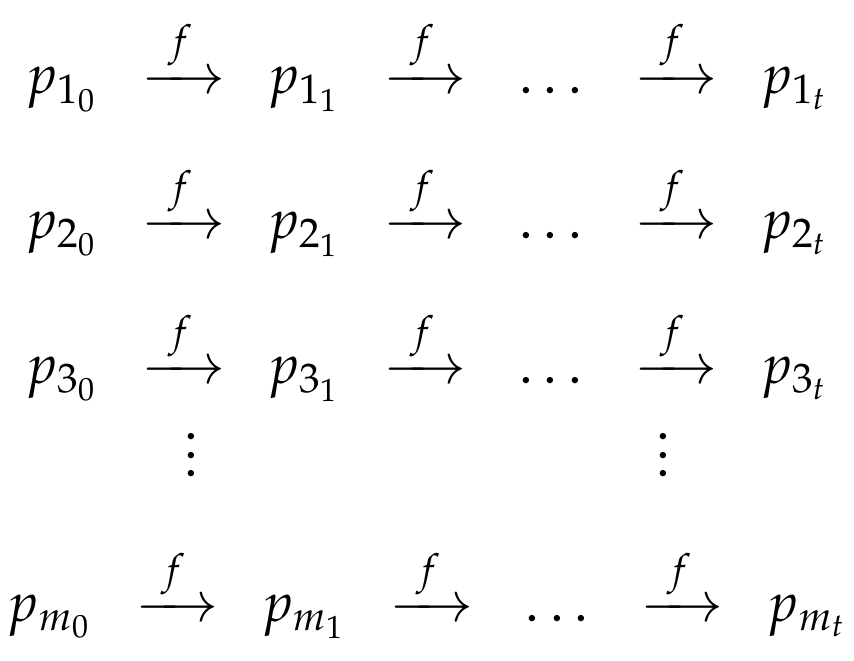
\includegraphics[scale = 0.38]{tabla.png}
    \caption{Computación esquematizada de las tablas de Hellman en su TMTO}
    \label{tabla}
\end{figure}
~\\

Una vez finalizado el proceso, no se almacenará la tabla en su totalidad, sino que tan sólo serán almacenadas la primera y última entradas de cada fila, formando una tupla. De tal forma, tomando el ejemplo anterior, se almacenarían las tuplas \{$p_{1_0}, h_{1_t}$\}, \{$p_{2_0}, h_{2_t}$\}, \{$p_{3_0}, h_{3_t}$\}, $~\dots$, \{$p_{m_0}, h_{m_t}$\}. Este almacenamiento se hace con el objetivo de ahorrar espacio en memoria.

\subsection{Empleando tablas para la búsqueda de colisiones}

A la hora de tratar de averiguar colisiones para la función \hash~atacada, con el objetivo de obtener una contraseña de forma ilegítima, se realizará el siguiente procedimiento. Habiendo obtenido un \hash~almacenado en el sistema, denominado $h$, el primer paso será compararlo con los \hashes~encontrados en las últimas columnas de la tabla, tras lo cual se pueden dar dos posibles situaciones, dependiendo de si $h$ colisiona con alguna de las últimas columnas:

\begin{itemize}

    \item \textbf{$h$ colisiona}: este caso puede darse si la contraseña correspondiente a $h$ se encuentra en la columna anterior de la tabla, o puede resultar en una falsa alarma. En ambos casos, como es conocida la fila en que ha aparecido $h$, se tomará su punto de inicio y desde él se repetirá el proceso de generación de la tabla, hasta llegar a la columna anterior a $h$, para la cual habrá de comprobarse si permite el acceso al sistema.
    \begin{itemize}
    
        \item \textbf{Acceso permitido}: efectivamente, se ha obtenido con éxito una de las contraseñas almacenadas en el sistema.
        
        \item \textbf{Acceso denegado}: falsa alarma. Esto sucede debido a que un valor \hash~puede ser obtenido aplicando la función correspondiente a diferentes contraseñas, por lo cual finalmente no se ha obtenido una contraseña válida.
        
    \end{itemize}

    \item \textbf{$h$ no colisiona}: en este caso, se aplicará la función de reconstrucción a $h$, seguida de la función \hash~empleada, obteniendo un nuevo \hash~$h'$, el cual vuelve a compararse con las últimas columnas de la tabla.
    
\end{itemize}

Puede ocurrir también que durante el proceso de generación de la tabla se generen colisiones el las últimas columnas, es decir, que dos o más de las últimas columnas acaben teniendo el mismo valor \hash. Esto contribuye a reducir el número de filas únicas de la tabla, aunque si se consigue mantener por debajo de un porcentaje pequeño no debería de tener un impacto negativo significante en la mejora brindada por el TMTO.

Hablando del cual, el intercambio tiempo-memoria que tiene lugar aquí depende de los valores asignados tanto a $m$ como a $t$. Una posible forma de pensar en dichos valores es tener en cuenta el número posible de \hashes~distintos que puede generar la función resumen atacada. Sea este número denominado $N$, una aproximación lógica trataría de asegurar que $m$ y $t$ cumplan la siguiente relación: $m \times t = N$. Dentro de esta relación, podrían darse los casos extremos de $m = N, t = 1$, o el contrario, $m = 1, t = N$, aunque dichos casos estarían implementando un ataque más parecido a la fuerza bruta en lugar de hacer uso del TMTO. En la época en la que Hellman ideó esta aproximación, en lugar de emplear tan sólo una tabla con dimensiones $m \times t = N$ su método hacía uso de diversas tablas de menor dimensionalidad para reducir las limitaciones establecidas por la memoria del sistema.

En el intercambio en este caso, un mayor número de filas respecto al número de columnas supondrá un menor tiempo de computación para la generación de la tabla, pero requerirá a su vez más espacio en memoria para almacenar los resultados, ya que se obtendrán más tuplas con la primera y última entrada de cada fila. En cambio, aumentar el valor de $t$ mientras se reduce el de $m$ resultará en una reducción en el espacio requerido en memoria, aunque el tiempo de computación necesario para obtener la tabla será mayor, ya que para cada fila se repetirá en procedimiento visto en la Figura \ref{tabla} un mayor número de veces. 

\chapter{El ataque del arco iris} \label{ataque}

\section{Desarrollo y relación con trabajos anteriores}

Hasta ahora se han visto diferentes aproximaciones cuyo objetivo recaía en la obtención de colisiones para una función resumen, para así poder tener acceso no autorizado a aquello que dicha función trataba de proteger. Aunque dichas aproximaciones no son empleadas hoy en día, sirvieron como base para el desarrollo del ataque del arco iris, el cual consiguió mejorar las prestaciones de todo lo visto anteriormente, mediante el uso de una estructura de datos que hace uso de los mismos principios que aquellos vistos en la Figura \ref{tabla}, expandiendo sobre ellos y resultando en las conocidas como tablas del arco iris.

En 2003, Philippe Oechslin publicó el primer artículo en el cual aparecía el concepto de la tabla del arco iris \cite{rainbow}. Dicha tabla consiste en una implementación más compleja del intercambio tiempo-memoria de Hellman, el cual se ha visto en la sección \ref{tmto}. Parte de la mayor complejidad se debe al aumento del tamaño de la tabla, ya que las limitaciones en cuanto a la memoria para almacenar las tablas que se daban lugar cuando Hellman publicó su artículo no ocurren en este caso.

\section{Tablas del arco iris: un viejo concepto revisitado}

La clave de este ataque reside en el uso de sus tablas, las cuales son capaces de representar mucha más información que las tablas que emplea Hellman. De hecho, el ataque llevado a cabo por Hellman requiere hacer uso de varias de sus tablas, mientras que si se pretende obtener los mismos resultados mediante tablas del arco iris únicamente haría falta emplear una de estas tablas. Las dimensiones de las tablas del arco iris dependerán, en principio, del número total de contraseñas diferentes a ser atacadas que existan, lo cual dependerá de las características de dichas contraseñas. Diferentes factores como el número de caracteres de las contraseñas o el uso o no de diferentes dominios de caracteres (letras minúsculas y/o mayúsculas, números, símbolos$\, \dots$) determinará las dimensiones de las tablas del arco iris. 

El método de construcción de las tablas del arco iris, como ya se ha dicho, sigue los mismos pasos de las tablas de Hellman, tomando una contraseñas inicial diferente para cada fila de la tabla, generando su valor \hash~y empleando la función de reconstrucción para obtener una nueva contraseña, así tantas veces como columnas tenga la tabla y para tantas filas como se requiera. Una vez generada una tabla del arco iris, será almacenada en memoria para su posterior uso. Dicho uso se llevará a cabo al igual que con las tablas de Hellman. La mejora en los resultados en este aspecto viene proporcionada por el aumento en las dimensiones de la tabla, aunque esto no es lo único que difiere en las tablas del arco iris.

\section{Propiedades fundamentales de las tablas del arco iris}

\subsection{Funciones de reconstrucción}

%Combinar diferentes funciones de reconstrucción
La característica más distinguida de las tablas del arco iris, y por la cual reciben su nombre, reside en el uso que son capaces de hacer de la función de reconstrucción, ya que es posible emplear diferentes funciones de reconstrucción en la misma tabla. Aunque esto no parezca tener demasiada importancia en un principio, en la práctica resulta ser un aspecto fundamental a la hora de obtener resultados de calidad, ya que estos variarán dependiendo de la función o funciones de reconstrucción empleadas. De esta manera, el foco de mayor importancia en cuanto a la construcción de tablas del arco iris se refiere pasa a ser la elección apropiada de una o varias funciones de reconstrucción, siendo el objetivo principal en este aspecto averiguar la configuración idónea de funciones de reconstrucción. 

\subsection{Escalabilidad}

Otra de las ventajas del ataque del arco iris es su escalabilidad, ya que una correcta implementación del mismo puede servir para atacar diferentes funciones \hash~y dominios de contraseñas. Las diferencias corresponderán únicamente con los tiempos empleado en la generación de las tablas y la búsqueda de contraseñas. A su vez, cabe la posibilidad de requerir ajustar las funciones de reconstrucción a las diferentes funciones \hash, aunque siempre dependerá del objetivo que se pretenda conseguir al buscar colisiones de la función correspondiente.

\section{Puntos distinguidos}

Dentro de las posibilidades que ofrece el ataque del arco iris en sí, existen también diferentes formas de llevarlo a cabo, siendo una variante muy popular el método de los puntos de control o puntos distinguidos, ideado por Rivest \cite{rivest}.

Tomando el método de Hellman \cite{hellman} mediante el uso del TMTO, Rivest implementó una mejora que reducía el tiempo de búsqueda a la hora de tratar de obtener contraseñas. Dicha mejora está basada en la implementación de puntos distinguidos en la tabla.

Los puntos distinguidos de Rivest se dan al establecer ciertas condiciones para las últimas entradas de la tabla, es decir, los elementos contenidos en las últimas columnas. Dichas condiciones quedan a la elección del atacante, pudiendo ser empezar o terminar con un número determinado de ceros o unos, por ejemplo. Esta aproximación tiene un matiz a la hora de generar la tabla, y es que como las últimas entradas deben cumplir las condiciones establecidas, ahora en lugar de obtener dichas entradas después de $t$ pasos, se habrá de continuar hasta generar una entrada que satisfaga dichas condiciones, lo cual puede darse en una entrada cercana a la inicial o puede tardar más de lo previsto en ocurrir. Por otra parte, la gran ventaja que brinda este método es una reducción significativa en cuanto al tiempo de búsqueda en las tablas, ya que el número de posibles colisiones de últimas entradas de la tabla se ve notablemente reducido, lo cual resulta también en un mayor rango de contraseñas cubierto por la tabla, aumentando la probabilidad de éxito de la misma.

\section{Contramedidas de una función \hash~para inutilizar el ataque del arco iris} \label{salt}

Aunque el ataque del arco iris tiene una efectividad muy alta cuando se implementa de la forma correcta, existen escenarios en los cuales resulta inviable implementar el ataque o directamente imposible, teniendo lugar mayormente cuando la función resumen la cual se pretende atacar hace uso de los siguientes métodos:

\begin{itemize}

    \item \textbf{\textit{Salting}}: la técnica conocida como \textit{salting} consiste en añadir una cadena aleatoria conocida como \textit{salt}, la cual no es secreta, a la contraseña antes de ser resumida, o directamente al valor \hash~resultante. Por ejemplo, si se partiera con la contraseña $p$, el \textit{salt} $s$ y la operación de concatenación $+$,~~sería posible obtener como valores \hash~ tanto $h = HASH(p+s)$ como $h = HASH(p)+s$. Para llevar a cabo el ataque del arco iris con éxito frente a funciones \hash~que hacen uso de esta técnica es necesario generar tablas del arco iris para cada \textit{salt} posible, lo cual para tamaños de \textit{salt} pequeños no supone un problema serio, pero en cuanto se alcanza cierto tamaño de \textit{salt} resulta inviable implementar el ataque debido a la enorme cantidad de tablas necesarias.
    
    \item \textbf{Estiramiento}: esta técnica hace uso del \textit{salting}, concatenándolo a la contraseña antes de generar el valor \hash~correspondiente. Tras obtener dicho \hash~se repite el mismo proceso un número de veces determinado, esta vez concatenando el \textit{salt} al valor \hash~antes obtenido. De esta forma, además de requerir tablas del arco iris para cada \textit{salt} posible, las tablas han de replicar el bucle de estiramiento, lo cual como es fácilmente observable puede resultar en la inviabilidad del ataque.
    
\end{itemize}

La aparición de estas técnicas consiguió dejar prácticamente inútil al ataque del arco iris, aunque incluso después de dicha aparición, los sistemas que no hacen uso del \textit{salting} o el estiramiento siguen siendo vulnerables a este ataque. Un ejemplo muy notorio pueden ser algunas versiones del sistema operativo \textit{Windows} de la empresa Microsoft, los cuales hasta el sistema \textit{Windows} 7 (incluido) han sido atacados con éxito por tablas del arco iris. De hecho, en su artículo original, Philippe Oechslin consigue con éxito romper el 100\% de las contraseñas almacenadas en los sistemas \textit{Windows} contra los que lanza su ataque \cite{rainbow}. Esto puede servir como muestra de la magnitud que llegó a alcanzar el ataque del arco iris.

\chapter{Experimentación}

Habiendo expuesto el funcionamiento del ataque del arco iris, así como los factores a tener en cuenta para su implementación, es el momento de detallar el desarrollo llevado a cabo. Dicho desarrollo, con el objetivo de encontrar colisiones para la función resumen atacada, simulará un ataque a las contraseñas de acceso a un sistema operativo, siendo el objetivo tratar de romper el máximo número de contraseñas posibles, para así conseguir de forma no autorizada acceder al sistema.

En primer lugar, se han de determinar dos aspectos fundamentales para el correcto funcionamiento del ataque: el dominio de contraseñas a atacar y la función \hash~que tratará de protegerlas.

\section{Especificaciones}

\subsection{Dominio de contraseñas atacado}

Un dominio de contraseñas puede ser descrito como todo el rango de posibles contraseñas válidas. En este caso, serán aquellas contraseñas que pueden emplearse para acceder al sistema operativo. Los factores que determinan un dominio son, fundamentalmente, la longitud de las contraseñas y los caracteres permitidos. En la implementación aquí desarrollada, las contraseñas tendrán una longitud exacta de seis caracteres, los cuales únicamente podrán ser números. Como resultado, el número total de contraseñas es de un millón, las cuales se encuentran en el rango $'000000',~\dots, '999999'$.

%Dominio, CRC-32, escalabilidad

\subsection{Función resumen atacada: CRC-32} \label{crc32}

Para este proyecto se ha escogido atacar valores \hash~de contraseñas generados utilizando la función \hash~CRC-32. Las siglas CRC provienen de \textit{cyclic redundancy check}, o lo que es lo mismo verificación por redundancia cíclica, mientras que el número 32 indica que las cadenas de salida resultantes tienen una longitud fija de 32 bits. Esta función pertenece a la familia de las funciones CRC, el uso de las cuales es bastante popular debido a su fácil implementación y rapidez de computación, entre otras cosas.

Cabe destacar que son de sobra conocidas las debilidades que presenta esta función \hash~a la hora de ocultar contraseñas frente a ataques criptográficos como el ataque del arco iris. De tal forma, se presupone que se obtendrán resultados satisfactorios al implementar el ataque frente a esta función.

Aunque en un primer momento tanto el dominio de contraseñas como la función resumen a atacar parezcan elecciones débiles, existe un motivo de peso para que así sea. Este desarrollo servirá para representar una implementación base, la cual es perfectamente escalable a dominios de contraseñas mayores y funciones \hash~más complejas. En el caso de una correcta implementación, el único aspecto que se verá afectado de forma más significativa sería el tiempo requerido para llevar a cabo el ataque, así como la memoria necesaria para almacenar las tablas del arco iris. De esta manera, debido a que será necesario experimentar con diversos tamaños de tabla y configuraciones de las mismas, los tiempos empleados y la memoria ocupada en disco en dicha experimentación serán mínimos, agilizando todo el proceso.

\section{Primera aproximación}

%R1, explicar diagonal, cribado en esquina inferior izquierda
\subsection{Dimensiones iniciales}

Como se ha visto en el apartado anterior, el dominio de contraseñas a ser atacadas consta de un total de un millón de contraseñas, el cual va a pasar a ser representado por el parámetro $N$. Como también sucediera anteriormente en la sección \ref{tmto} al introducir el intercambio tiempo-memoria (TMTO), en la generación de tablas al implementar el ataque del arco iris se ha de tener en cuenta el tamaño de dichas tablas, el cual depende de el número total de contraseñas. Recuérdese que el tamaño de una tabla en el ataque del arco iris viene dado por el número de filas ($m$) y de columnas ($t$) que posee. Una de las mayores diferencias de este ataque respecto al TMTO de Hellman es que así como en el TMTO se hacía uso de diversas tablas de menor dimensión, en el ataque del arco iris basta con generar una sola tabla de mayor dimensionalidad. En este caso, el tamaño de la tabla debería de cumplir:

\begin{center}
    \begin{equation}
        \tag{Fórmula 1}
        m \times t \approx 10^6 = N
        \label{tamaño}
    \end{equation}
\end{center}

Teniendo esto en cuenta, se procederá a generar diferentes tablas de tamaños diversos, la mayoría cumpliendo con la relación establecida en la \ref{tamaño}, aunque algunas tablas tendrán tamaños por encima o por debajo de $N$, para explorar más posibilidades y observar la eficiencia de las tablas con diferentes tamaños, algunos cumpliendo con la \ref{tamaño} y otros no. Aunque los tamaños de tabla empleados se verán más adelante, los posibles valores para $m$ y $t$ serán los siguientes:

\begin{itemize}

    \item $m \in $\{250, 500, 1.000, 2.000, 2.500, 5.000, 10.000, 20.000, \\
    25.000, 50.000, 100.000, 200.000, 250.000, 500.000, 1.000.000\}
    
    \item $t \in $\{1, 2, 4, 5, 10, 20, 40, 50, 100, 200, 400, 500, 1.000\}
    
\end{itemize}

Aunque inicialmente existirán muchos tamaños de tabla, el objetivo será determinar a partir de qué tamaños se obtienen resultados satisfactorios, para así poner el foco sobre aquellos tamaños para los cuales no se haya podido romper tantas contraseñas como se deseaba en un principio. De esta forma, se pretende averiguar los tamaños de tabla más eficientes que consigan romper el máximo número de contraseñas. En este caso la eficiencia de una tabla viene medida en términos de memoria necesaria para su almacenamiento y tiempo requerido para su generación y búsqueda de contraseñas.

\subsection{Función de reconstrucción}

Queda todavía por especificar la función de reconstrucción a emplear. Cabe recordar que una función de reconstrucción toma como entrada una valor \hash, y produce como salida una contraseña dentro del dominio $N$. Inicialmente la función de reconstrucción elegida, la cual pasará a denominarse \textbf{R1} desde este instante, actuaba de manera muy eficiente. Su comportamiento se ve a continuación, haciendo uso un valor \hash~$h$ y su correspondiente reconstrucción $r$:

\begin{itemize}

	\item tomando $h$ en forma numérica, esta función le aplicará la operación módulo un millón, con el objetivo de obtener los seis últimos números de $h$. Partiendo desde una contraseña $p = $~'112233', y su correspondiente valor \hash~$h = $~'3570655599', la función de reconstrucción \textbf{R1} sigue el siguiente proceso:

		\begin{enumerate}

			\item Una vez obtenido el valor \hash~$h = $~'3570655599', se le aplicará la operación módulo un millón, con el objetivo de obtener los últimos seis dígitos del \hash.

			\item La reconstrucción resultante será $r = $~'655599', la cual pertenece al dominio de contraseñas $N$.

		\end{enumerate}

\end{itemize}

\subsection{Generación y uso de tablas del arco iris}

Una vez se ha especificado el dominio de contraseñas, la función \hash~a atacar y la función de reconstrucción a emplear, es momento de establecer el método de generación de las tablas del arco iris. Para ello, inicialmente será necesario elegir las dimensiones $m \times t$ de la tabla a generar, y posteriormente, como se ha visto en la Figura \ref{tabla}, una vez determinados los parámetros $m$ (filas) y $t$ (columnas), los pasos a seguir en este caso serán:

\begin{enumerate}[label*=\arabic*.]

    \item Tomar una contraseña inicial $p$
    
    \item Obtener $h$, el valor \hash~de $p$
    
    \begin{enumerate}[label*=\arabic*.]
    
        \item Reconstruir $h$, obteniendo $r$
        
        \item Generar $h$ de nuevo, siendo el valor \hash~de $r$
        
        \item Repetir $t$ veces
        
    \end{enumerate}
    
    \item Guardar $p$ y el último $h$ obtenido en la tabla
    
    \item Repetir $m$ veces
    
\end{enumerate}

La tabla del arco iris resultante será almacenada en memoria, aunque con unas dimensiones reducidas respecto a las empleadas en su generación. Mientras que el número de filas de cada tabla seguirá siendo $m$, el número de columnas se ve reducido, guardando tan sólo dos columnas por cada fila, las cuales corresponderán con la primera y la última columna de cada fila obtenidas durante la construcción de la tabla. No es necesario almacenar la tabla en su totalidad, ya que al emplear funciones de reconstrucción deterministas -es decir, que siempre generan el mismo resultado para cada entrada específica- únicamente se requiere saber desde qué contraseña inicial se ha partido en cada fila para volver a generarla en su totalidad siguiendo el proceso descrito en los pasos 1, 2, 3 y 4 arriba vistos.

Cabe destacar que las contraseñas iniciales para cada fila se irán tomando del dominio en orden de valor ascendente. De esta manera, la contraseña inicial para la primera fila de la tabla siempre será $p_{1_0} = $'000000', mientras que la contraseña inicial para la segunda fila de la tabla será $p_{2_0} = $'000001', y así sucesivamente.

Recuérdese que se está tratando de romper contraseñas almacenadas en forma de valores \hash. La manera de conseguirlo será si, durante el proceso de generación de una tabla, se llega a obtener dicho \hash~que se está tratando de romper, ya que eso significará que la entrada anterior en la tabla será su contraseña correspondiente. A la hora de buscar contraseñas en una tabla, antes que nada se buscará en las entradas guardadas en memoria, ya que si el valor \hash~se encuentra en una de las últimas entradas de la tabla no hay necesidad de volver a generarla, debido a que se puede concluir que es posible obtener su contraseña correspondiente. En caso de no encontrar el valor \hash~en una de las últimas entradas de la tabla, se realizará el proceso de búsqueda volviendo a generar la tabla, ya que cabe la posibilidad de que el valor \hash~a romper se encuentre en una de las entradas entre la primera y la última, las cuales no han sido almacenadas en memoria. Si en algún momento durante esta búsqueda se da con el valor \hash~a romper, se concluye la búsqueda con éxito. El caso opuesto significará que la tabla no ha sido capaz de romper esa contraseña.

En cuanto a el tamaño de la tabla, puede observarse que cuantas más filas posea, mayor probabilidad existirá de romper una contraseña sin necesidad de generar la tabla de nuevo, mientras que cuantas más columnas tenga una tabla, generará un mayor número de posibles contraseñas en la búsqueda, por lo cual aumentará la probabilidad de romper una contraseña con éxito. Viendo estas propiedades, es muy tentador generar tablas del máximo tamaño posible, ya que en principio parece que parten con ventaja respecto a tablas más pequeñas. Bien, no todo son ventajas con un mayor tamaño, ya que si bien la probabilidad de éxito aumenta, también lo hace en principio el porcentaje de colisiones en una misma tabla. Una colisión se da cuando para filas diferentes de una tabla, el valor \hash~generado en la última entrada es el mismo, resultando en una reducción del número de contraseñas únicas cubiertas por la tabla. También en cuanto al tamaño, si bien en este caso es factible construir tablas que contengan todas las contraseñas, ya que son en total $N = 10^6$, en el momento en que se esté tratando con un dominio de contraseñas de mayor tamaño esta posibilidad queda eliminada, ya que sería inviable obtener dichas tablas debido al tiempo requerido en su construcción y/o la memoria requerida para almacenarlas. En este caso las tablas con un millón de entradas no tardan más de cinco minutos en ser generadas y ocupan un total de 22.0 MB en memoria, siendo perfectamente viables.

\subsection{Último ajuste: la estructura de datos}

Antes de proceder a las pruebas de este primer lote de tablas del arco iris, queda detallar el aspecto final de la implementación del ataque del arco iris. En cuanto han sido determinados todos los parámetros que configurarán las tablas del arco iris, únicamente falta elegir la estructura de datos que será empleada para representarlas, la cual queda a elección del atacante. A la hora de optar por una estructura de datos u otra, se ha de tener en cuenta, como ya ha sido mencionado anteriormente, que no se va a almacenar en memoria la tabla en su totalidad, es decir, todas las $m \times t$ entradas, sino que únicamente se almacenarán la primera y última entradas de cada fila de la tabla, o lo que es lo mismo, la primera y última columnas de cada fila. Dentro de todas las posibilidades lo ideal sería, una vez que se haya desarrollado el método de construcción de tablas, generar aquellas que se desee mediante diferentes estructuras de datos, para una vez obtenidas todas ellas comparar los tiempos necesarios en su construcción y en el acceso a las mismas, así como el espacio que ocupan en memoria. En el caso de la implementación aquí desarrollada, se compararon tablas del arco iris representadas mediante listas de tuplas y diccionarios. Cada una de estas estructuras de datos representa las tablas de la siguiente forma:

\begin{itemize}

    \item \textbf{Lista de tuplas}: Cada entrada de la lista corresponde a una fila de la tabla y contiene una tupla o pareja de elementos. El primero de estos elementos es la contraseña inicial de la fila correspondiente, mientras que el segundo elemento corresponde al valor \hash~obtenido en la última entrada de la fila correspondiente. De esta manera, empleando la Figura \ref{tabla} como ejemplo, la lista de tuplas que equivaldría a esta tabla del arco iris correspondería con la siguiente representación: [($p_{1_0}, h_{1_t}$),~($p_{2_0}, h_{2_t}$),~($p_{3_0}, h_{3_t}$), ~$\dots$,~($p_{m_0}, h_{m_t}$)].
    
    \item \textbf{Diccionario}: esta estructura de datos viene como anillo al dedo a la hora de representar tablas del arco iris, debido a su estructura interna siendo cada entrada compuesta de una clave y su valor correspondiente, tal que \textit{clave : valor}. De tal forma, en cada entrada del diccionario correspondiente a una fila de la tabla, la \textit{clave} será igual a la primera contraseña de dicha fila, mientras que el \textit{valor} corresponderá con el resumen \hash~generado en la última columna de dicha fila. De nuevo, si se toma como ejemplo la Figura \ref{tabla}, el diccionario resultante que representaría a la tabla del arco iris correspondiente sería el siguiente: \{$p_{1_0} : h_{1_t},~p_{2_0} : h_{2_t},~p_{3_0} : h_{3_t}, ~\dots,~p_{m_0} : h_{m_t}$\}.
    
\end{itemize}

Tras construir las primeras tablas del arco iris de diversos tamaños, habiendo generado dos copias de cada una, siendo una copia representada por una lista de tuplas y la otra por un diccionario, se experimentó con ellas midiendo los tiempos empleados en la generación y búsqueda, así como la memoria ocupada. Tras realizar dicha experimentación, se optó por elegir el diccionario como estructura de datos para todas las futuras tablas. Esto fue debido a que, si bien los tiempos requeridos por cada una de las estructuras de datos resultaron ser extremadamente similares, las tablas representadas por un diccionario ocupaban cerca de la mitad del espacio en memoria que aquellas de igual tamaño pero guardadas en forma de lista de tuplas.

Una vez establecido todo lo necesario para construir las tablas del arco iris, se puede proceder a su generación y almacenamiento en disco, para así tenerlas preparadas para llevar a cabo el ataque contra las contraseñas de acceso al sistema, las cuales hay que generar también.

\subsection{Generación de contraseñas de acceso} \label{contraseñas}

Para simular las contraseñas almacenadas en un sistema operativo en forma de valores \hash, se generarán un total de 1.000 valores \hash~aleatorios. Para su obtención se escogerá de forma aleatoria 1.000 contraseñas contenidas en el dominio establecido ($N$), generando el valor \hash~correspondiente de cada una y almacenándolo en una lista. Dicha lista será almacenada en disco al finalizar el proceso de obtención del los 1.000 valores \hash. Las contraseñas correspondientes a estos 1.000 \hashes~serán las que todas las tablas tratarán de romper, es decir, obtener la contraseña original únicamente conociendo el valor \hash~correspondiente.

\subsection{Primeras pruebas}\label{primeras pruebas}

Una vez generadas todas las tablas del arco iris y las contraseñas a atacar, es el momento de ponerse manos a la obra. A cada tabla empleada en el ataque del arco iris a las contraseñas se le asigna un porcentaje de éxito. Dicho porcentaje de éxito para cada tabla se mide dividiendo el número de contraseñas que ha sido capaz de romper entre el número total de contraseñas a romper, 1.000 en este caso. Para todos los resultados se empleará el mismo código de color indicando la calidad de los mismos:

\begin{itemize}

    \item \textcolor{red}{rojo}: porcentaje de éxito en el rango de 0,~$\dots$,~69'99\%.
    
    \item \textcolor{y}{amarillo}: porcentaje de éxito en el rango de 70,~$\dots$,~84'99\%.
    
    \item \textcolor{b}{azul}: porcentaje de éxito en el rango de 85,~$\dots$,~94'99\%.
    
    \item \textcolor{g}{verde}: porcentaje de éxito en el rango de 95,~$\dots$,~100\%.
    
\end{itemize}

Idealmente se desea que las tablas del arco iris generadas sean capaces de romper todas las contraseñas almacenadas en el sistema. Si bien esto es posible en este caso para el dominio de contraseñas elegido, si se expandiese dicho dominio resultaría más complicado, por lo cual si una tabla consigue romper al menos 950 contraseñas de las 1.000 generadas aleatoriamente será clasificada como idónea. Así mismo, una tabla que no llegue a romper tantas contraseñas pero consiga al menos adivinar 850 será clasificada como aceptable, ya que significará que en la mayoría de los casos será capaz de acceder al sistema. Las tablas que no consigan llegar a ese nivel no serían válidas para ser empleadas en un ataque, aunque si al menos consiguen romper 700 contraseñas puede considerarse que se han quedado cerca de ser aceptables, mientras que una tabla que ni siquiera consiga romper 700 contraseñas debería de ser descartada de inmediato, ya que tendría una probabilidad de adivinar una contraseña similar a sacar cara o cruz tirando una moneda al aire.

Los resultados de la primera prueba pasan a verse a continuación, con las tablas que emplean la función de reconstrucción \textbf{R1}:

\def\arraystretch{1.5}
\begin{table}[H]
	\LARGE
	\centering
	\resizebox{\textwidth}{!}{\begin{tabular}{|c|r|c|c|c|c|c|c|c|c|c|c|c|c|c|}
		\hline
		\multirow{13}{*}{$t$} & 1 & & & & & & & & & & & & & \textcolor{g}{100\%} \\ \cline{2-15}
		& 2 & & & & & & & & & & & & \textcolor{b}{91.9\%} & \\ \cline{2-15}
		& 4 & & & & & & & & & & & \textcolor{b}{90.6\%} & & \\ \cline{2-15}
		& 5 & & & & & & & & & & \textcolor{b}{90.6\%} & & & \\ \cline{2-15}
		& 10 & & & & & & & & & \textcolor{g}{95.2\%} & & & & \\ \cline{2-15}
		& 20 & & & & & & & & \textcolor{g}{96.1\%} & & & & & \\ \cline{2-15}
		& 40 & & & & & & & \textcolor{g}{97.1\%} & & & & & & \\ \cline{2-15}
		& 50 & & & & & & \textcolor{g}{97.4\%} &  & \textcolor{g}{99.3\%} & \textcolor{g}{99.6\%} & & \textcolor{g}{99.6\%} & \textcolor{g}{100\%} & \textcolor{g}{100\%} \\ \cline{2-15}
		& 100 & & & & & \textcolor{g}{96.4\%} & \textcolor{g}{98.0\%} & \textcolor{g}{98.4\%} & \textcolor{g}{99.0\%} & \textcolor{g}{99.8\%} & & \textcolor{g}{100\%} & \textcolor{g}{100\%} & \textcolor{g}{100\%} \\ \cline{2-15}
		& 200 & & & & \textcolor{g}{95.2\%} & & & & & & & & & \\ \cline{2-15}
		& 400 & & & \textcolor{b}{91.8\%} & & & & & & & & & & \\ \cline{2-15}
		& 500 & & \textcolor{y}{84.1\%} & & & & & & & & & & & \\ \cline{2-15}
		& 1000 & \textcolor{r}{63.5\%} & & & & & & & & & & & & \\ \cline{2-15}
		& & 1000 & 2000 & 2500 & 5000 & 10000 & 20000 & 25000 & 50000 & 100000 & 200000 & 250000 & 500000 & 1000000 \\ \hline
		& & \multicolumn{13}{|c|}{$m$} \\ \hline
	\end{tabular}}
	\caption{Porcentajes de éxito para las tablas empleando \textbf{R1}}
	\label{resR1}
\end{table}

Puede observarse que en este caso se obtienen resultados bastante satisfactorios. Tan sólo una de las tablas sería descartada, aquella con dimensiones 1000 $\times$ 1000, mientras que después de esa solamente hay otra que no llega a ser aceptable, aunque se queda realmente cerca de conseguirlo. Todas las tablas con 2500 filas o más serán consideradas como aceptables o idóneas, llegando incluso a obtener un éxito del 100\% en varios casos, si bien dichas tablas tienen unas dimensiones que exceden el dominio elegido. Por ejemplo, la primera tabla que consigue un porcentaje de éxito perfecto tiene unas dimensiones de 250.000 $\times$ 100 = 25.000.000 $>$ 1.000.000 $= N$. Es interesante también observar como para las tablas con mayor número de filas, si se intenta mantener unas dimensiones dentro del dominio $N$ resultan peores que tablas con menos filas pero más profundidad. Por ejemplo, la tabla con dimensiones 200.000 $\times$ 5 tiene menor porcentaje de éxito que la tabla con dimensiones 20.000 $\times$ 50, teniendo un 10\% de las filas, pero 10 veces la profundidad, lo cual resulta clave para su mejor resultado.

Los resultados obtenidos pueden servir para confirmar que el desarrollo llevado a cabe de la implementación del ataque del arco iris ha sido correcto, ya que la mayoría de las tablas generadas brindan excelentes resultados. Aún así, resultaría interesante experimentar con una función de reconstrucción diferente, con el objetivo de mejorar los resultados.

\section{Una nueva función de reconstrucción}

Así como la función de reconstrucción empleada en la sección anterior (\textbf{R1}) actúa sobre el valor numérico del \hash generado por la función CRC-32, esta nueva función de reconstrucción, la cual pasará a denominarse \textbf{R2}, actuará sobre el valor en hexadecimal del \hash, aunque también hace uso de su valor numérico. Al igual que ya se hizo con \textbf{R1}, a continuación se mostrará el comportamiento de la nueva función de reconstrucción \textbf{R2}, haciendo uso de una valor \hash~$h$ y su correspondiente reconstrucción $r$:

\begin{itemize}

	\item tomando $h$ en forma hexadecimal, esta función inicialmente eliminará los dos primeros caracteres de $h$, los cuales siempre serán '0x'. Seguidamente, mientras el \hash~resultante tenga una longitud mayor a seis caracteres, se irá eliminando el primero de estos caracteres, hasta obtener una longitud igual a seis. Por último, todas las letras que queden en $h$ serán sustituidas por números. Estos números no serán seleccionados al azar, sino que corresponderán con los números de $h$ en forma numérica, comenzando desde el final, y tras cada sustitución se tomará el número anterior. Partiendo desde una contraseña $p =$~'112233', y su correspondiente valor \hash~hexadecimal $h =$~'0xd4d3e16f', la función de reconstrucción \textbf{R2} sigue el siguiente proceso:

		\begin{enumerate}
				
			\item Obtener primero los valores \hash~en forma numérica ~$h_{num} =$'3570655599' y en forma hexadecimal $h_{hex} =$~'0xd4d3e16f'

			\item Eliminar los dos primeros caracteres de $h_{hex}$, resultando en $h_{hex} =$~'d4d3e16f'.
		
			\item Mientras la longitud de $h_{hex}$ sea mayor que seis, eliminar su primer carácter, resultando finalmente en $h_{hex} =$~'d3e16f'
		
			\item Recorrer los caracteres de $h_{hex}$ desde el principio, y aquellos que sean letras se reemplazan por números de $h_{num}$ comenzando por el final. Tras este paso se tendrá $r = '939165'$, ya que se habrán sustituido las letras 'd', 'e' y 'f' por los números $9, 9$ y $5$, los cuales se encuentran en la última, penúltima y antepenúltima posición de $h_{num}$, respectivamente.

		\end{enumerate}

\end{itemize}

Una vez especificado el comportamiento de esta nueva función de reconstrucción, de nuevo es momento de generar tablas del arco iris que hagan uso de ella, para tratar de atacar las mismas contraseñas que las tablas anteriores.

\subsection{Nuevos resultados}

En esta ocasión, el tamaño de las tablas generadas será el mismo que en el apartado \ref{primeras pruebas}, para así poder comprobar de manera sencilla la diferencia entre ambas implementaciones. Los resultados obtenidos con la función de reconstrucción \textbf{R2} son los siguientes:

\def\arraystretch{1.5}
\begin{table}[H]
	\LARGE
	\centering
	\resizebox{\textwidth}{!}{\begin{tabular}{|c|r|c|c|c|c|c|c|c|c|c|c|c|c|c|}
		\hline
		\multirow{13}{*}{$t$} & 1 & & & & & & & & & & & & & \textcolor{g}{100\%} \\ \cline{2-15}
		& 2 & & & & & & & & & & & & \textcolor{b}{91.1\%} & \\ \cline{2-15}
		& 4 & & & & & & & & & & & \textcolor{b}{89.4\%} & & \\ \cline{2-15}
		& 5 & & & & & & & & & & \textcolor{b}{88.8\%} & & & \\ \cline{2-15}
		& 10 & & & & & & & & & \textcolor{b}{93.0\%} & & & & \\ \cline{2-15}
		& 20 & & & & & & & & \textcolor{g}{95.5\%} & & & & & \\ \cline{2-15}
		& 40 & & & & & & & \textcolor{g}{97.1\%} & & & & & & \\ \cline{2-15}
		& 50 & & & & & & \textcolor{g}{97.1\%} &  & \textcolor{g}{98.8\%} & \textcolor{g}{99.7\%} & & \textcolor{g}{100\%} & \textcolor{g}{100\%} & \textcolor{g}{100\%} \\ \cline{2-15}
		& 100 & & & & & \textcolor{g}{97.1\%} & \textcolor{g}{98.8\%} & \textcolor{g}{99.2\%} & \textcolor{g}{99.6\%} & \textcolor{g}{99.9\%} & & \textcolor{g}{99.9\%} & \textcolor{g}{99.9\%} & \textcolor{g}{100\%} \\ \cline{2-15}
		& 200 & & & & \textcolor{b}{94.3\%} & & & & & & & & & \\ \cline{2-15}
		& 400 & & & \textcolor{y}{82.1\%} & & & & & & & & & & \\ \cline{2-15}
		& 500 & & \textcolor{y}{74.9\%} & & & & & & & & & & & \\ \cline{2-15}
		& 1000 & \textcolor{r}{57.1\%} & & & & & & & & & & & & \\ \cline{2-15}
		& & 1000 & 2000 & 2500 & 5000 & 10000 & 20000 & 25000 & 50000 & 100000 & 200000 & 250000 & 500000 & 1000000 \\ \hline
		& & \multicolumn{13}{|c|}{$m$} \\ \hline
	\end{tabular}}
	\caption{Porcentajes de éxito para las tablas empleando \textbf{R2}}
	\label{resR2}
\end{table}

Observando en un primer vistazo la distribución de los colores a lo largo de la tabla se puede apreciar que los resultados aquí obtenidos son peores que los anteriores en la tabla \ref{resR1} con la función de reconstrucción \textbf{R1}. La tabla del arco iris que ya se esperaba que fuera a ser descartada con $m =$ 1.000 rinde peor que antes, y se han generado menos tablas idóneas que en los resultados anteriores. De nuevo, las tablas con un número de entradas muy elevado siguen alcanzando el 100\% de porcentaje de éxito. Con todo esto siguen siendo resultados satisfactorios, ya que hay múltiples tablas con un porcentaje de éxito mayor al 95\%.

Aunque no se esperaba un empeoramiento en la calidad de los resultados, siguen siendo satisfactorios en general. Hasta ahora tan sólo se ha hecho uso de una función de reconstrucción en las tablas del arco iris. Una vez visto esto, es el momento de tratar de combinarlas con el objetivo de obtener mejores resultados, explotando esta característica fundamental de las tablas del arco iris.

\section{Combinando funciones de reconstrucción}

\subsection{Combinación básica}

Habiendo ya empleado ambas funciones de reconstrucción, \textbf{R1} y \textbf{R2}, la forma más intuitiva de combinarlas en una misma tabla del arco iris consiste en concatenar su uso. De esta manera, para cada fila de la tabla, para la primera entrada o columna la utilizará la función de reconstrucción \textbf{R1}, mientras que para la entrada siguiente se hará uso de la función \textbf{R2}, y así sucesivamente. Tomando como referencia la Figura \ref{tabla}, la construcción de cada fila de las tablas del arco iris configuradas con la concatenación de funciones de reconstrucción corresponderá con el siguiente esquema, para una columna $c$:

 \begin{figure}[H]

	\centering

	$p_{1_c}~ \xrightarrow{CRC-32}~ h_{1_c}~ \xrightarrow{\textbf{R1}}~ r_{1_c}~ \xrightarrow{CRC-32}~ h_{2_c}~ \xrightarrow{\textbf{R2}}~ r_{2_c}~ \xrightarrow{CRC-32}~ h_{3_c}~ \xrightarrow{\textbf{R1}}~ r_{3_c} \dots$ \\

	\caption{Generación de una fila concatenando funciones de reconstrucción}
	\label{filaR1R2}
	 
 \end{figure}

El rendimiento de estas tablas contra las contraseñas de acceso al sistema es el siguiente:

\def\arraystretch{1.5}
\begin{table}[H]
	\LARGE
	\centering
	\resizebox{\textwidth}{!}{\begin{tabular}{|c|r|c|c|c|c|c|c|c|c|c|c|c|c|c|}
		\hline
		\multirow{13}{*}{$t$} & 1 & & & & & & & & & & & & & \textcolor{g}{100\%} \\ \cline{2-15}
		& 2 & & & & & & & & & & & & \textcolor{g}{97.0\%} & \\ \cline{2-15}
		& 4 & & & & & & & & & & & \textcolor{g}{96.2\%} & & \\ \cline{2-15}
		& 5 & & & & & & & & & & \textcolor{g}{97.0\%} & & & \\ \cline{2-15}
		& 10 & & & & & & & & & \textcolor{g}{98.3\%} & & & & \\ \cline{2-15}
		& 20 & & & & & & & & \textcolor{g}{99.5\%} & & & & & \\ \cline{2-15}
		& 40 & & & & & & & \textcolor{g}{99.7\%} & & & & & & \\ \cline{2-15}
		& 50 & & & & & & \textcolor{g}{99.6\%} &  & \textcolor{g}{100\%} & \textcolor{g}{100\%} & & \textcolor{g}{100\%} & \textcolor{g}{100\%} & \textcolor{g}{100\%} \\ \cline{2-15}
		& 100 & & & & & \textcolor{g}{99.9\%} & \textcolor{g}{99.9\%} & \textcolor{g}{99.9\%} & \textcolor{g}{100\%} & \textcolor{g}{100\%} & & \textcolor{g}{100\%} & \textcolor{g}{100\%} & \textcolor{g}{100\%} \\ \cline{2-15}
		& 200 & & & & \textcolor{g}{99.9\%} & & & & & & & & & \\ \cline{2-15}
		& 400 & & & \textcolor{g}{98.1\%} & & & & & & & & & & \\ \cline{2-15}
		& 500 & & \textcolor{g}{95.4\%} & & & & & & & & & & & \\ \cline{2-15}
		& 1000 & \textcolor{r}{63.1\%} & & & & & & & & & & & & \\ \cline{2-15}
		& & 1000 & 2000 & 2500 & 5000 & 10000 & 20000 & 25000 & 50000 & 100000 & 200000 & 250000 & 500000 & 1000000 \\ \hline
		& & \multicolumn{13}{|c|}{$m$} \\ \hline
	\end{tabular}}
	\caption{Porcentajes de éxito para las tablas empleando la concatenación de las funciones de reconstrucción}
	\label{resR1R2}
\end{table}

Estos son los mejores resultados obtenidos hasta el momento debido a que, aunque todavía existe la misma tabla descartable con 1.000 entradas, el resto de tablas del arco iris generadas son idóneas, habiendo obtenido incluso un mayor número de tablas que han conseguido romper todas las contraseñas. Entrando en detalle en las tablas perfectas, además de las tablas más grandes de las cuales ya se esperaban estos resultados, se puede observar que la tabla con dimensiones 50.000$\times$50 es la de menor tamaño entre ellas, lo cual significa que sería la que menos memoria requiriese para ser almacenada. De esta tabla se podría decir también que sería, dentro de aquellas con un éxito del 100\%, una de las que menos tiempo requeriría en su generación, ya que si bien posee un número elevado de columnas, sus pocas filas en comparación a las demás reducirán el tiempo para construirla.

De esta manera ha quedado reflejada la utilidad de poder combinar diferentes funciones de reconstrucción en una misma tabla del arco iris. Teniendo en cuenta que esta combinación de ambas funciones de reconstrucción es la más simple de todas, resultaría interesante saber si una combinación más intrincada proporcionaría mejores resultados.

\subsection{Una combinación algo más compleja}

Siguiendo el mismo comportamiento que la combinación anterior, surge una nueva con un ligero cambio. En esta ocasión, en lugar de concatenar ambas funciones, se establecerá un patrón cíclico, el cual seguirá el siguiente comportamiento: se empleará \textbf{R1}en la primera reconstrucción de cada fila, mientras que para las siguientes dos reconstrucciones se hará uso de \textbf{R2}. Acto seguido se volverá a usar \textbf{R1}, repitiendo este patrón hasta alcanzar el final la fila correspondiente. Tomando el esquema de la Figura \ref{filaR1R2}, haciendo uso de nuevo de una columna $c$, el método de generación de una fila para las tablas del arco iris que sigan esta configuración será el siguiente:

\begin{figure}[H]
	
	\centering

	$p_{1_c}~ \xrightarrow{CRC-32}~ h_{1_c}~ \xrightarrow{\textbf{R1}}~ r_{1_c}~ \xrightarrow{CRC-32}~ h_{2_c}~ \xrightarrow{\textbf{R2}}~ r_{2_c}~ \dots$ \\
	~\\
	$\dots~\xrightarrow{CRC-32}~ h_{3_c}~ \xrightarrow{\textbf{R2}}~ r_{3_c}~\xrightarrow{CRC-32}~ h_{4_c}~ \xrightarrow{\textbf{R1}}~ r_{4_c}~\dots$

	\caption{Generación de una fila combinando funciones de reconstrucción mediante un patrón reducido}
	\label{filapp}

\end{figure}

El ataque del arco iris llevado a cabo con las tablas que hacen uso de este patrón de reconstrucción obtienen los siguientes resultados:

\def\arraystretch{1.5}
\begin{table}[H]
	\LARGE
	\centering
	\resizebox{\textwidth}{!}{\begin{tabular}{|c|r|c|c|c|c|c|c|c|c|c|c|c|c|c|}
		\hline
		\multirow{13}{*}{$t$} & 1 & & & & & & & & & & & & & \textcolor{g}{100\%} \\ \cline{2-15}
		& 2 & & & & & & & & & & & & \textcolor{b}{83.7\%} & \\ \cline{2-15}
		& 4 & & & & & & & & & & & \textcolor{b}{82.6\%} & & \\ \cline{2-15}
		& 5 & & & & & & & & & & \textcolor{b}{86.0\%} & & & \\ \cline{2-15}
		& 10 & & & & & & & & & \textcolor{b}{88.8\%} & & & & \\ \cline{2-15}
		& 20 & & & & & & & & \textcolor{b}{92.9\%} & & & & & \\ \cline{2-15}
		& 40 & & & & & & & \textcolor{g}{96.2\%} & & & & & & \\ \cline{2-15}
		& 50 & & & & & & \textcolor{g}{97.8\%} &  & \textcolor{g}{99.5\%} & \textcolor{g}{99.8\%} & & \textcolor{g}{100\%} & \textcolor{g}{100\%} & \textcolor{g}{100\%} \\ \cline{2-15}
		& 100 & & & & & \textcolor{g}{97.8\%} & \textcolor{g}{99.4\%} & \textcolor{g}{99.8\%} & \textcolor{g}{99.9\%} & \textcolor{g}{100\%} & & \textcolor{g}{100\%} & \textcolor{g}{100\%} & \textcolor{g}{100\%} \\ \cline{2-15}
		& 200 & & & & \textcolor{g}{96.7\%} & & & & & & & & & \\ \cline{2-15}
		& 400 & & & \textcolor{b}{90.1\%} & & & & & & & & & & \\ \cline{2-15}
		& 500 & & \textcolor{b}{87.2\%} & & & & & & & & & & & \\ \cline{2-15}
		& 1000 & \textcolor{y}{71.3\%} & & & & & & & & & & & & \\ \cline{2-15}
		& & 1000 & 2000 & 2500 & 5000 & 10000 & 20000 & 25000 & 50000 & 100000 & 200000 & 250000 & 500000 & 1000000 \\ \hline
		& & \multicolumn{13}{|c|}{$m$} \\ \hline
	\end{tabular}}
	\caption{Porcentajes de éxito para las tablas empleando el patrón reducido}
	\label{respp}
\end{table}

Por primera vez no se han generado tablas que vayan a ser descartadas. Incluso la tabla que habitualmente tiene el peor rendimiento ($m =$ 1.000) en esta ocasión ha quedado significativamente cerca de ser considerada aceptable. Aunque este patrón es algo más complejo que la concatenación anteriormente vista, por lo cual se esperaba generar mejores resultados, no ha sido suficiente para proporcionar la mejora esperada frente a la configuración anterior. El esquema general vuelva a ocurrir aquí también, con las tablas ya esperadas teniendo un porcentaje de éxito del 100\%.

Tras observar estos resultados, cabe la posibilidad de que al nuevo patrón le falta la complejidad necesaria para llegar a mejorar los resultados. Habiendo llegado a este punto es necesario descartar esa posibilidad.

\subsection{La combinación final, la más compleja}

En esta ocasión se va a emplear un método similar al anteriormente expuesto, aunque se va a complicar un poco más. En lugar de emplear un patrón que se repite cada tres pasos, la longitud del mismo casi se triplicará. Al igual que en el anterior patrón, se comenzará empleado \textbf{R1} para la primera entrada, mientras que para las siguientes dos entradas se hará uso de la función de reconstrucción \textbf{R2}. Tras estos tres primeros pasos, los dos siguientes emplearán la función de reconstrucción \textbf{R1}.Por último, para los tres pasos finales se utiliza de nuevo \textbf{R2}. De nuevo, para una columna $c$ de la tabla, el método de generación de una fila corresponderá con el siguiente esquema:

\begin{figure}[H]
	
	\centering

	$p_{1_c}~ \xrightarrow{CRC-32}~ h_{1_c}~ \xrightarrow{\textbf{R1}}~ r_{1_c}~ \xrightarrow{CRC-32}~ h_{2_c}~ \xrightarrow{\textbf{R2}}~ r_{2_c}~ \xrightarrow{CRC-32}~ h_{3_c}~ \xrightarrow{\textbf{R2}}~ r_{3_c} \dots$ \\
	~\\
	$\dots \xrightarrow{CRC-32}~ h_{4_c}~ \xrightarrow{\textbf{R1}}~ r_{4_c}~ \xrightarrow{CRC-32}~ h_{5_c}~ \xrightarrow{\textbf{R1}}~ r_{5_c}~ \xrightarrow{CRC-32}~ h_{6_c}~ \xrightarrow{\textbf{R2}}~ r_{6_c} \dots$ \\
	~\\
	$\dots \xrightarrow{CRC-32}~ h_{7_c}~ \xrightarrow{\textbf{R2}}~ r_{7_c}~ \xrightarrow{CRC-32}~ h_{8_c}~ \xrightarrow{\textbf{R2}}~ r_{8_c}~ \xrightarrow{CRC-32}~ h_{9_c}~\xrightarrow{\textbf{R1}}~ \dots$\;\;\;\; \\

	\caption{Generación de una fila combinando funciones de reconstrucción mediante un patrón extenso}
	\label{filaPG}

\end{figure}

Los resultados tras aplicar el ataque del arco iris con las tablas que hacen uso de esta configuración son los siguientes:

\def\arraystretch{1.5}
\begin{table}[H]
	\LARGE
	\centering
	\resizebox{\textwidth}{!}{\begin{tabular}{|c|r|c|c|c|c|c|c|c|c|c|c|c|c|c|}
		\hline
		\multirow{13}{*}{$t$} & 1 & & & & & & & & & & & & & \textcolor{g}{100\%} \\ \cline{2-15}
		& 2 & & & & & & & & & & & & \textcolor{b}{84.7\%} & \\ \cline{2-15}
		& 4 & & & & & & & & & & & \textcolor{b}{83.0\%} & & \\ \cline{2-15}
		& 5 & & & & & & & & & & \textcolor{b}{82.2\%} & & & \\ \cline{2-15}
		& 10 & & & & & & & & & \textcolor{b}{87.3\%} & & & & \\ \cline{2-15}
		& 20 & & & & & & & & \textcolor{b}{89.3\%} & & & & & \\ \cline{2-15}
		& 40 & & & & & & & \textcolor{b}{93.8\%} & & & & & & \\ \cline{2-15}
		& 50 & & & & & & \textcolor{g}{95.6\%} &  & \textcolor{g}{99.9\%} & \textcolor{g}{99.9\%} & & \textcolor{g}{100\%} & \textcolor{g}{100\%} & \textcolor{g}{100\%} \\ \cline{2-15}
		& 100 & & & & & \textcolor{g}{95.9\%} & \textcolor{g}{99.2\%} & \textcolor{g}{99.5\%} & \textcolor{g}{99.8\%} & \textcolor{g}{100\%} & & \textcolor{g}{100\%} & \textcolor{g}{100\%} & \textcolor{g}{100\%} \\ \cline{2-15}
		& 200 & & & & \textcolor{g}{96.0\%} & & & & & & & & & \\ \cline{2-15}
		& 400 & & & \textcolor{b}{92.2\%} & & & & & & & & & & \\ \cline{2-15}
		& 500 & & \textcolor{b}{90.4\%} & & & & & & & & & & & \\ \cline{2-15}
		& 1000 & \textcolor{r}{60.4\%} & & & & & & & & & & & & \\ \cline{2-15}
		& & 1000 & 2000 & 2500 & 5000 & 10000 & 20000 & 25000 & 50000 & 100000 & 200000 & 250000 & 500000 & 1000000 \\ \hline
		& & \multicolumn{13}{|c|}{$m$} \\ \hline
	\end{tabular}}
	\caption{Porcentajes de éxito para las tablas empleando el patrón extenso}
	\label{resPG}
\end{table}

Estos resultados son peores que los obtenidos anteriormente tanto por el patrón reducido como por la concatenación de funciones de reconstrucción. Empleando el patrón extenso se esperaba en principio una mejora en los resultados. Si bien estos son mejores que los obtenidos por las tablas que hacen uso de tan sólo una función de reconstrucción, aunque no en la medida esperada, es aparente que los resultados no suponen una mejora respecto a las tablas vistas en la Tabla \ref{resR1R2}. En este caso también se obtienen tablas capaces de romper todas las contraseñas, las cuales ya vienen siendo habituales para los tamaños correspondientes, aunque se pueden observar un mayor número de tabla aceptables pero no idóneas.

\section{En busca de la configuración perfecta} \label{config perf}

Tras la primera tanda de pruebas, es fácilmente observable que, para tablas que superen las 10.000 filas, el porcentaje de éxito no baja del 88.0\%. Dichas tablas serán capaces de romper la gran mayoría de las contraseñas almacenadas en el sistema. Si bien esta es la intención del ataque del arco iris, resultaría interesante indagar en tablas de menor tamaño, para así poder determinar si realmente es necesario crear tablas que contengan tantas filas, o si por el contrario existen ciertas configuraciones que son capaces de brindar resultados igual de buenos que las tablas más grandes. Encontrar dichas configuraciones es de gran interés, ya que de ser posible conseguirlo significaría una reducción en los requerimientos tanto de tiempo como de memoria, algo que siempre es beneficioso en este tipo de ataques.

\subsection{Nuevos tamaños} \label{nuevos_tamaños}

Si bien en las pruebas anteriores la tabla con un menor número de filas poseía $m =$ 1.000 filas, en la búsqueda de las tablas con resultados similares a los mejores obtenidos anteriormente pero con menor tamaño será necesario emplear tamaños de tabla diferentes, expandiendo la búsqueda con tamaños menores a los vistos anteriormente. De tal forma, la tabla con menos filas pasará a tener $m = 250$, mientras que la tabla más grande tendrá $m =$ 10.000 filas. En concreto, se generarán tantas tablas como posibles permutaciones existan de los siguientes conjuntos de $m$ y $t$:
\\
\begin{itemize}

    \item $m \in$ \{250, 500, 750, 1.000, 1.500, 2.000, 2.500, 5.000, 10.000\}
    
    \item $t \in$ \{50, 100, 200, 400, 500, 1.000\}
    
\end{itemize}

\subsection{Colisiones de las nuevas tablas}

En total se generarán $6 \cdot 9 = 54$ tablas para cada combinación de funciones de reconstrucción. Tras generar todas estas tablas, pero antes de obtener su rendimiento, resulta de interés observar las colisiones dichas tablas en las diferentes combinaciones de funciones de reconstrucción. Para ello se obtendrá el porcentaje de colisiones de cada tabla, obteniendo primero el número de colisiones recorriendo sus últimas columnas, determinando cuántos de sus valores no se repiten y asignando esa cantidad a un valor $c$, para seguidamente restarlo al número total de filas de la tabla ($m$), siendo el resultado de esta operación el número de colisiones de la tabla. Acto seguido dicho número de colisiones será dividido entre el número de filas de la tabla ($m$), dando como resultado el porcentaje de colisiones de la tabla. Para dichos porcentajes, al igual que se ha hecho anteriormente con los porcentajes de éxito, se empleará un código de color, el cual será el siguiente:

\begin{itemize}

    \item \textcolor{red}{rojo}: porcentaje de colisiones en el rango de 70,~$\dots$, 100\%.
    
    \item \textcolor{y}{amarillo}: porcentaje de colisiones en el rango de 50,~$\dots$, 69'99\%.
    
    \item \textcolor{b}{azul}: porcentaje de colisiones en el rango de 25,~$\dots$, 49'99\%.

    \item \textcolor{g}{verde}: porcentaje de colisiones en el rango de 0,~$\dots$, 24'99\%.
    
\end{itemize}

Interpretando este código de color podría decirse que una tabla que tengan colisiones en un 70 por ciento de sus filas o más no serían las más ideales para ser empleadas en la búsqueda de contraseñas, ya que tantas colisiones se traducen en una reducción muy significante de las contraseñas cubiertas por esa tabla. Si este porcentaje se reduce un poco, mientras una tabla cubra cerca de la mitad de sus contraseñas, serán sus dimensiones las que determinen su utilidad, ya que si la tabla es lo suficientemente grande será capaz de compensar la pérdida de contraseñas cubiertas con su tamaño. Cualquier tabla que cubra más de la mitad de sus contraseñas será aceptable en este aspecto, aunque de nuevo sus dimensiones serán cruciales para determinar su efectividad atacando contraseñas. Por último, todas aquellas tablas que cubran tres cuartas partes o más de las contraseñas que se pretenden serán en principio las más efectivas.

Comenzando al igual que antes por las tablas que tan sólo emplean la reconstrucción con la operación módulo un millón (\textbf{R1}), se obtiene:

\def\arraystretch{1.5}
\begin{table}[H]
	\centering
	\resizebox{\textwidth}{!}{\begin{tabular}{|c|r|c|c|c|c|c|c|c|c|c|}
		\hline
		\multirow{6}{*}{$t$} & 50 & \textcolor{g}{0.80\%} & \textcolor{g}{1.80\%} & \textcolor{g}{2.40\%} & \textcolor{g}{2.60\%} & \textcolor{g}{4.27\%} & \textcolor{g}{5.15\%} & \textcolor{g}{5.80\%} & \textcolor{g}{10.16\%} & \textcolor{g}{19.08\%} \\ \cline{2-11}
		& 100 & \textcolor{g}{2.00\%} & \textcolor{g}{2.60\%} & \textcolor{g}{4.00\%} & \textcolor{g}{5.00\%} & \textcolor{g}{7.47\%} & \textcolor{g}{9.55\%} & \textcolor{g}{10.76\%} & \textcolor{g}{18.96\%} & \textcolor{b}{32.75\%} \\ \cline{2-11}
		& 200 & \textcolor{g}{3.60\%} & \textcolor{g}{4.60\%} & \textcolor{g}{6.80\%} & \textcolor{g}{8.90\%} & \textcolor{g}{13.00\%} & \textcolor{g}{16.00\%} & \textcolor{g}{17.92\%} & \textcolor{b}{30.60\%} & \textcolor{b}{47.18\%} \\ \cline{2-11}
		& 400 & \textcolor{g}{5.20\%} & \textcolor{g}{8.40\%} & \textcolor{g}{13.07\%} & \textcolor{g}{16.50\%} & \textcolor{g}{23.47\%} & \textcolor{b}{28.55\%} & \textcolor{b}{31.96\%} & \textcolor{b}{48.74\%} & \textcolor{y}{65.83\%} \\ \cline{2-11}
		& 500 & \textcolor{g}{6.00\%} & \textcolor{g}{10.00\%} & \textcolor{g}{15.20\%} & \textcolor{g}{19.40\%} & \textcolor{b}{27.00\%} & \textcolor{b}{32.55\%} & \textcolor{b}{36.68\%} & \textcolor{y}{54.74\%} & \textcolor{r}{71.14\%} \\ \cline{2-11}
		& 1000 & \textcolor{g}{9.20\%} & \textcolor{g}{13.60\%} & \textcolor{g}{18.93\%} & \textcolor{g}{24.00\%} & \textcolor{b}{33.20\%} & \textcolor{b}{40.35\%} & \textcolor{b}{45.68\%} & \textcolor{y}{65.02\%} & \textcolor{r}{79.64\%} \\ \hline
		& & 250 & 500 & 750 & 1000 & 1500 & 2000 & 2500 & 5000 & 10000 \\ \hline
		& & \multicolumn{9}{c|}{$m$} \\ \hline
	\end{tabular}}
	\caption{Porcentajes de colisiones para las tablas empleando \textbf{R1}}
	\label{colR1}
\end{table}

Como era de esperar y va a ser habitual en estos resultados, las tablas con menos filas tendrán porcentajes de colisiones menores respecto a las tablas de mayor tamaño. Las únicas tablas con un porcentaje de colisiones muy restrictivo ocurren con unas dimensiones superiores al dominio $N$, lo cual no es sorprendente en tales casos. Se puede concluir que es uso exclusivo de \textbf{R1}, en cuanto a colisiones, parece prometer resultados satisfactorios a la hora de atacar contraseñas.

Para las tablas que emplean únicamente la función de reconstrucción utilizando el \hash~en hexadecimal (\textbf{R2}) se obtienen los siguientes resultados:

\def\arraystretch{1.5}
\begin{table}[H]
	\centering
	\resizebox{\textwidth}{!}{\begin{tabular}{|c|r|c|c|c|c|c|c|c|c|c|}
		\hline
		\multirow{6}{*}{$t$} & 50 & \textcolor{g}{0.00\%} & \textcolor{g}{1.60\%} & \textcolor{g}{2.00\%} & \textcolor{g}{2.60\%} & \textcolor{g}{4.20\%} & \textcolor{g}{5.70\%} & \textcolor{g}{6.64\%} & \textcolor{g}{12.52\%} & \textcolor{g}{22.60\%} \\ \cline{2-11}
		& 100 & \textcolor{g}{0.40\%} & \textcolor{g}{2.60\%} & \textcolor{g}{4.27\%} & \textcolor{g}{5.50\%} & \textcolor{g}{8.13\%} & \textcolor{g}{10.15\%} & \textcolor{g}{12.32\%} & \textcolor{g}{22.50\%} & \textcolor{b}{36.42\%} \\ \cline{2-11}
		& 200 & \textcolor{g}{2.80\%} & \textcolor{g}{7.20\%} & \textcolor{g}{9.47\%} & \textcolor{g}{12.40\%} & \textcolor{g}{16.27\%} & \textcolor{g}{18.80\%} & \textcolor{g}{21.60\%} & \textcolor{b}{34.72\%} & \textcolor{y}{51.27\%} \\ \cline{2-11}
		& 400 & \textcolor{g}{11.60\%} & \textcolor{g}{18.00\%} & \textcolor{g}{21.73\%} & \textcolor{b}{27.10\%} & \textcolor{b}{34.13\%} & \textcolor{b}{38.75\%} & \textcolor{b}{43.28\%} & \textcolor{y}{58.74\%} & \textcolor{r}{73.00\%} \\ \cline{2-11}
		& 500 & \textcolor{g}{15.60\%} & \textcolor{g}{23.60\%} & \textcolor{b}{27.60\%} & \textcolor{b}{33.40\%} & \textcolor{b}{41.07\%} & \textcolor{b}{46.50\%} & \textcolor{y}{51.68\%} & \textcolor{y}{67.52\%} & \textcolor{r}{79.88\%} \\ \cline{2-11}
		& 1000 & \textcolor{g}{18.00\%} & \textcolor{b}{28.80\%} & \textcolor{b}{35.87\%} & \textcolor{b}{42.80\%} & \textcolor{y}{53.67\%} & \textcolor{y}{60.95\%} & \textcolor{y}{66.76\%} & \textcolor{r}{81.62\%} & \textcolor{r}{90.47\%} \\ \hline
		& & 250 & 500 & 750 & 1000 & 1500 & 2000 & 2500 & 5000 & 10000 \\ \hline
		& & \multicolumn{9}{c|}{$m$} \\ \hline
	\end{tabular}}
	\caption{Porcentajes de colisiones para las tablas empleando \textbf{R2}}
	\label{colR2}
\end{table}

En esta ocasión, aunque para las tablas de menor tamaño se obtiene un menor número de colisiones, en cuanto aumentan las dimensiones de las tablas los resultados empeoran respecto a los anteriores. Esta es la razón por la cual, como se ha visto en las primeras pruebas, estas tablas tienen un peor rendimiento que las que emplean únicamente \textbf{R1}, aunque aún así seguían siendo buenos resultados. En este caso se han generado más tablas con peores porcentajes de colisiones, la más grande de ellas superando el 90 por ciento de colisiones, lo que se traduce en menos de 1.000 contraseñas cubiertas por una tabla que en principio se esperaba que cubriese 10.000. También hay más tablas por encima del cincuenta por ciento, cubriendo algo menos de la mitad de las contraseñas previstas, lo cual considerando su tamaño puede llegar a comprometer su rendimiento de manera significativa.

Pasando ahora a las tablas que combinan ambas funciones de reconstrucción se obtiene:

\def\arraystretch{1.5}
\begin{table}[H]
	\centering
	\resizebox{\textwidth}{!}{\begin{tabular}{|c|r|c|c|c|c|c|c|c|c|c|}
		\hline
		\multirow{6}{*}{$t$} & 50 & \textcolor{g}{0.80\%} & \textcolor{g}{1.00\%} & \textcolor{g}{1.73\%} & \textcolor{g}{2.30\%} & \textcolor{g}{3.93\%} & \textcolor{g}{5.30\%} & \textcolor{g}{6.32\%} & \textcolor{g}{11.48\%} & \textcolor{g}{20.74\%} \\ \cline{2-11}
		& 100 & \textcolor{g}{0.80\%} & \textcolor{g}{1.60\%} & \textcolor{g}{3.07\%} & \textcolor{g}{4.30\%} & \textcolor{g}{6.80\%} & \textcolor{g}{8.80\%} & \textcolor{g}{10.96\%} & \textcolor{g}{19.48\%} & \textcolor{b}{33.78\%} \\ \cline{2-11}
		& 200 & \textcolor{g}{2.00\%} & \textcolor{g}{4.80\%} & \textcolor{g}{6.67\%} & \textcolor{g}{8.30\%} & \textcolor{g}{12.60\%} & \textcolor{g}{16.65\%} & \textcolor{g}{20.00\%} & \textcolor{b}{32.16\%} & \textcolor{b}{49.08\%} \\ \cline{2-11}
		& 400 & \textcolor{g}{2.40\%} & \textcolor{g}{9.00\%} & \textcolor{g}{12.80\%} & \textcolor{g}{17.80\%} & \textcolor{g}{23.00\%} & \textcolor{b}{29.05\%} & \textcolor{b}{33.24\%} & \textcolor{b}{47.44\%} & \textcolor{y}{63.71\%} \\ \cline{2-11}
		& 500 & \textcolor{g}{3.20\%} & \textcolor{g}{11.00\%} & \textcolor{g}{16.13\%} & \textcolor{g}{21.80\%} & \textcolor{b}{27.33\%} & \textcolor{b}{33.60\%} & \textcolor{b}{38.24\%} & \textcolor{y}{52.96\%} & \textcolor{y}{68.54\%} \\ \cline{2-11}
		& 1000 & \textcolor{g}{9.60\%} & \textcolor{g}{21.40\%} & \textcolor{b}{29.20\%} & \textcolor{b}{36.90\%} & \textcolor{b}{46.00\%} & \textcolor{y}{53.40\%} & \textcolor{y}{59.24\%} & \textcolor{r}{74.32\%} & \textcolor{r}{85.00\%} \\ \hline
		& & 250 & 500 & 750 & 1000 & 1500 & 2000 & 2500 & 5000 & 10000 \\ \hline
		& & \multicolumn{9}{c|}{$m$} \\ \hline
	\end{tabular}}
	\caption{Porcentajes de colisiones para las tablas empleando la concatenación de las funciones de reconstrucción}
	\label{colR1R2}
\end{table}

Aunque se ha mejorado respecto a las tablas que emplean únicamente \textbf{R2}, en comparación a las primeras tablas que hacen uso tan sólo de \textbf{R1} existen más colisiones en estas tablas, aunque en general estos resultados no son mucho peores. Este pequeño empeoramiento resulta sorprendente, ya que se esperaba que al combinar ambas funciones de reconstrucción el porcentaje de colisiones fuera reducido drásticamente. En línea con lo anteriormente visto siguen tanto la distribución de colores a lo largo de la tabla como los altos porcentajes de las tablas de mayor tamaño. Aún con todo, estos resultados se podrían clasificar como satisfactorios.

Para las tablas que emplean el denominado patrón reducido (\textbf{R1 + R2 + R2}) se generan los siguientes resultados:

\def\arraystretch{1.5}
\begin{table}[H]
	\centering
	\resizebox{\textwidth}{!}{\begin{tabular}{|c|r|c|c|c|c|c|c|c|c|c|}
		\hline
		\multirow{6}{*}{$t$} & 50 & \textcolor{g}{0.80\%} & \textcolor{g}{0.60\%} & \textcolor{g}{0.80\%} & \textcolor{g}{1.10\%} & \textcolor{g}{1.73\%} & \textcolor{g}{2.00\%} & \textcolor{g}{2.68\%} & \textcolor{g}{4.86\%} & \textcolor{g}{9.30\%} \\ \cline{2-11}
		& 100 & \textcolor{g}{1.20\%} & \textcolor{g}{1.40\%} & \textcolor{g}{2.13\%} & \textcolor{g}{2.70\%} & \textcolor{g}{3.53\%} & \textcolor{g}{4.35\%} & \textcolor{g}{5.56\%} & \textcolor{g}{9.08\%} & \textcolor{g}{16.16\%} \\ \cline{2-11}
		& 200 & \textcolor{g}{1.60\%} & \textcolor{g}{2.00\%} & \textcolor{g}{2.80\%} & \textcolor{g}{3.80\%} & \textcolor{g}{5.40\%} & \textcolor{g}{6.75\%} & \textcolor{g}{8.44\%} & \textcolor{g}{14.32\%} & \textcolor{b}{25.46\%} \\ \cline{2-11}
		& 400 & \textcolor{g}{2.00\%} & \textcolor{g}{4.00\%} & \textcolor{g}{5.07\%} & \textcolor{g}{6.70\%} & \textcolor{g}{9.87\%} & \textcolor{g}{12.70\%} & \textcolor{g}{15.44\%} & \textcolor{g}{24.70\%} & \textcolor{b}{39.64\%} \\ \cline{2-11}
		& 500 & \textcolor{g}{1.60\%} & \textcolor{g}{3.80\%} & \textcolor{g}{5.73\%} & \textcolor{g}{7.40\%} & \textcolor{g}{11.47\%} & \textcolor{g}{14.65\%} & \textcolor{g}{17.80\%} & \textcolor{b}{29.54\%} & \textcolor{b}{45.17\%} \\ \cline{2-11}
		& 1000 & \textcolor{g}{5.60\%} & \textcolor{g}{11.80\%} & \textcolor{g}{16.13\%} & \textcolor{g}{18.90\%} & \textcolor{b}{25.87\%} & \textcolor{b}{30.75\%} & \textcolor{b}{35.08\%} & \textcolor{y}{51.08\%} & \textcolor{y}{67.09\%} \\ \hline
		& & 250 & 500 & 750 & 1000 & 1500 & 2000 & 2500 & 5000 & 10000 \\ \hline
		& & \multicolumn{9}{c|}{$m$} \\ \hline
	\end{tabular}}
	\caption{Porcentajes de colisiones para las tablas empleando el patrón reducido}
	\label{colpp}
\end{table}

De nuevo se obtienen unos resultados que no cumplen con lo inicialmente esperado en ciertos aspectos. Con el uso de este patrón se esperaba reducir el número de colisiones respecto a tabla que empleasen tan sólo \textbf{R1} o \textbf{R2}, lo cual como puede observarse ocurre con claridad. Las tablas que emplean este patrón reducido poseen el menor número de colisiones, llegando incluso a no existir ninguna tabla con más de un 67\% de colisiones. Tan sólo nueve tablas de las 54 totales en este caso superan el 25 por ciento de colisiones, y de estas únicamente dos pasan del 50 por ciento. Sin duda alguna estos son los mejores resultados en cuanto a colisiones se refiere.

Por último, en cuanto a las tablas que emplean el denominado patrón extenso (\textbf{R1 + R2 + R2 + R1 + R1 + R2 + R2 + R2}) se observan los siguientes resultados:

\def\arraystretch{1.5}
\begin{table}[H]
	\centering
	\resizebox{\textwidth}{!}{\begin{tabular}{|c|r|c|c|c|c|c|c|c|c|c|}
		\hline
		\multirow{6}{*}{$t$} & 50 & \textcolor{g}{0.00\%} & \textcolor{g}{0.40\%} & \textcolor{g}{0.67\%} & \textcolor{g}{0.80\%} & \textcolor{g}{1.27\%} & \textcolor{g}{1.70\%} & \textcolor{g}{2.04\%} & \textcolor{g}{3.18\%} & \textcolor{g}{6.70\%} \\ \cline{2-11}
		& 100 & \textcolor{g}{1.20\%} & \textcolor{g}{1.20\%} & \textcolor{g}{1.60\%} & \textcolor{g}{2.30\%} & \textcolor{g}{3.93\%} & \textcolor{g}{4.80\%} & \textcolor{g}{5.60\%} & \textcolor{g}{11.20\%} & \textcolor{g}{20.63\%} \\ \cline{2-11}
		& 200 & \textcolor{g}{2.40\%} & \textcolor{g}{4.60\%} & \textcolor{g}{7.87\%} & \textcolor{g}{9.50\%} & \textcolor{g}{14.67\%} & \textcolor{g}{17.55\%} & \textcolor{g}{20.28\%} & \textcolor{b}{33.68\%} & \textcolor{y}{50.76\%} \\ \cline{2-11}
		& 400 & \textcolor{g}{4.00\%} & \textcolor{g}{8.00\%} & \textcolor{g}{12.80\%} & \textcolor{g}{16.50\%} & \textcolor{g}{23.53\%} & \textcolor{b}{28.25\%} & \textcolor{b}{32.44\%} & \textcolor{b}{48.94\%} & \textcolor{y}{65.97\%} \\ \cline{2-11}
		& 500 & \textcolor{g}{3.60\%} & \textcolor{g}{4.60\%} & \textcolor{g}{7.87\%} & \textcolor{g}{10.20\%} & \textcolor{g}{15.73\%} & \textcolor{g}{18.80\%} & \textcolor{g}{22.12\%} & \textcolor{b}{36.64\%} & \textcolor{y}{54.28\%} \\ \cline{2-11}
		& 1000 & \textcolor{g}{10.40\%} & \textcolor{g}{21.80\%} & \textcolor{b}{30.80\%} & \textcolor{b}{36.80\%} & \textcolor{b}{45.33\%} & \textcolor{y}{51.30\%} & \textcolor{y}{55.88\%} & \textcolor{r}{70.64\%} & \textcolor{r}{82.47\%} \\ \hline
		& & 250 & 500 & 750 & 1000 & 1500 & 2000 & 2500 & 5000 & 10000 \\ \hline
		& & \multicolumn{9}{c|}{$m$} \\ \hline
	\end{tabular}}
	\caption{Porcentajes de colisiones para las tablas empleando el patrón extenso}
	\label{colPG}
\end{table}

Puede observarse como las tablas con esta configuración poseen menor número de colisiones que las anteriores en la Tabla \ref{colR1R2} (\textbf{R1 + R2}), lo cual era de esperar, ya que el objetivo de establecer este patrón era forzar una reducción en el número de colisiones. Lo sorprendente en esta caso es que siguen habiendo porcentajes de colisiones mayores que en la Tabla \ref{colR1} (\textbf{R1}). Esto resulta totalmente inesperado, ya que la función de reconstrucción \textbf{R1} parece en principio la más simple, dando a entender que sería la que más colisiones produciría, empeorando los resultados. Otro hecho sorprendente en este caso es que las tablas que emplean el patrón reducido resulten mejores en cuanto al porcentaje de colisiones respecto al patrón extenso, siendo esta mejora más que notable. Una cosa queda clara, y es que el objetivo inicial de emplear este patrón no se ha cumplido, aunque resta por ver la efectividad de estas tablas a la hora de tratar de romper contraseñas.

\section{Resultados finales}

Habiendo obtenido los porcentajes de colisiones para las tablas con cada una de las combinaciones de funciones de reconstrucción es el momento de realizar el ataque del arco iris con ellas. De esta forma se espera determinar qué tamaño de tabla es el ideal en cuanto a contraseñas rotas, tiempo empleado en su generación y memoria requerida para su almacenamiento. En principio lo más lógico sería esperar que las tablas con menor número de colisiones fueran las que mejor rendimiento tuvieran, ya que cuantas menos colisiones se den lugar en una tabla mayor será el número de contraseñas cubiertas por esa tabla. Siguiendo esta lógica, las tablas con mayor éxito deberían de ser las que hacen uso del patrón reducido (\textbf{R1 + R2 + R2}), ya que presentan una diferencia significante en sus porcentajes de colisiones, como se ha visto en la Tabla \ref{colpp}.

Como ya se ha hecho anteriormente en el apartado \ref{primeras pruebas}, cada una de las tablas que se pretende analizar tendrá la tarea de atacar las mismas contraseñas aleatorias generadas en el apartado \ref{contraseñas}, obteniendo el porcentaje de contraseñas rotas respecto al total de contraseñas a romper.

Comenzando como es habitual por las tablas que tan sólo hacen uso de la función de reconstrucción con la operación módulo un millón (\textbf{R1}) se obtienen los siguientes resultados:

\def\arraystretch{1.5}
\begin{table}[H]
	\centering
	\resizebox{\textwidth}{!}{\begin{tabular}{|c|r|c|c|c|c|c|c|c|c|c|}
		\hline
		\multirow{6}{*}{$t$} & 50 & \textcolor{r}{14.6\%} & \textcolor{r}{27.9\%} & \textcolor{r}{39.0\%} & \textcolor{r}{46.6\%} & \textcolor{r}{59.4\%} & \textcolor{r}{67.8\%} & \textcolor{y}{73.8\%} & \textcolor{b}{87.4\%} & \textcolor{b}{94.7\%} \\ \cline{2-11}
		& 100 & \textcolor{r}{22.1\%} & \textcolor{r}{41.9\%} & \textcolor{r}{55.8\%} & \textcolor{r}{65.8\%} & \textcolor{y}{77.2\%} & \textcolor{y}{81.6\%} & \textcolor{b}{85.9\%} & \textcolor{b}{92.3\%} & \textcolor{g}{96.4\%} \\ \cline{2-11}
		& 200 & \textcolor{r}{24.0\%} & \textcolor{r}{46.2\%} & \textcolor{r}{61.2\%} & \textcolor{y}{71.3\%} & \textcolor{y}{81.6\%} & \textcolor{b}{87.7\%} & \textcolor{b}{91.0\%} & \textcolor{g}{95.2\%} & \textcolor{g}{97.7\%} \\ \cline{2-11}
		& 400 & \textcolor{r}{23.7\%} & \textcolor{r}{45.0\%} & \textcolor{r}{60.5\%} & \textcolor{r}{69.9\%} & \textcolor{y}{82.1\%} & \textcolor{b}{88.5\%} & \textcolor{b}{91.8\%} & \textcolor{g}{96.0\%} & \textcolor{g}{98.3\%} \\ \cline{2-11}
		& 500 & \textcolor{r}{23.5\%} & \textcolor{r}{44.3\%} & \textcolor{r}{58.2\%} & \textcolor{r}{67.0\%} & \textcolor{y}{78.3\%} & \textcolor{y}{84.1\%} & \textcolor{b}{87.9\%} & \textcolor{b}{94.6\%} & \textcolor{g}{97.9\%} \\ \cline{2-11}
		& 1000 & \textcolor{r}{22.7\%} & \textcolor{r}{42.4\%} & \textcolor{r}{55.1\%} & \textcolor{r}{63.5\%} & \textcolor{y}{72.7\%} & \textcolor{y}{77.6\%} & \textcolor{y}{80.7\%} & \textcolor{b}{86.2\%} & \textcolor{b}{89.3\%} \\ \hline
		& & 250 & 500 & 750 & 1000 & 1500 & 2000 & 2500 & 5000 & 10000 \\ \hline
		& & \multicolumn{9}{c|}{$m$} \\ \hline
	\end{tabular}}
	\caption{Porcentajes de éxito para las tablas que emplean \textbf{R1}}
	\label{exR1}
\end{table}

Como era de esperar, las tablas de menor tamaño no realizan un buen trabajo a la hora de adivinar contraseñas. Aunque dichas tablas tenían porcentajes de colisiones realmente bajos, puede observarse ahora como esa característica no es suficiente para romper muchas contraseñas. Hace falta que las tablas posean al menos 1.000 filas para comenzar a ser efectivas, y una vez superan las 2.000 filas los resultados encontrados son en su mayoría satisfactorios. En esta ocasión no se han generado tablas con efectividad perfecta, es decir, con un porcentaje de éxito del 100\%, aunque algunas tablas se han quedado a las puertas de conseguirlo.

Es interesante también observar que la profundidad ideal para las tablas con esta configuración es de 400 columnas para las tablas con más de 1.000 filas, lo cual muestra como una mayor profundidad de tabla no se traduce en un porcentaje de éxito más elevado. Esto es debido a que cuanto más se aumenta la profundidad de una tabla más veces se genera el valor \hash~de una contraseña para ser reconstruido a continuación, con lo cual aumenta la probabilidad de generar colisiones en la tabla, reduciendo el número de contraseñas cubiertas por dicha tabla, resultando en un menor porcentaje de éxito.

Viendo estos resultados, si se pretende emplear la tabla de menor tamaño posible que sea aceptable a la hora de romper contraseñas, habría de emplearse la tabla de dimensiones $m =$ 2.000, $t =$ 200, mientras que los mejores resultados los brinda la tabla de dimensiones $m =$ 10.000, $t =$ 400.

Pasando ahora a las tablas que emplean únicamente la función de reconstrucción con el \hash~en hexadecimal (\textbf{R2}) se obtienen los siguientes resultados:

\def\arraystretch{1.5}
\begin{table}[H]
	\centering
	\resizebox{\textwidth}{!}{\begin{tabular}{|c|r|c|c|c|c|c|c|c|c|c|}
		\hline
		\multirow{6}{*}{$t$} & 50 & \textcolor{r}{15.9\%} & \textcolor{r}{29.7\%} & \textcolor{r}{40.2\%} & \textcolor{r}{48.8\%} & \textcolor{r}{61.2\%} & \textcolor{r}{69.7\%} & \textcolor{y}{76.0\%} & \textcolor{b}{88.6\%} & \textcolor{b}{94.4\%} \\ \cline{2-11}
		& 100 & \textcolor{r}{22.2\%} & \textcolor{r}{41.7\%} & \textcolor{r}{56.2\%} & \textcolor{r}{66.2\%} & \textcolor{y}{76.9\%} & \textcolor{y}{82.8\%} & \textcolor{b}{87.0\%} & \textcolor{b}{93.4\%} & \textcolor{g}{97.1\%} \\ \cline{2-11}
		& 200 & \textcolor{r}{24.1\%} & \textcolor{r}{44.4\%} & \textcolor{r}{61.2\%} & \textcolor{y}{70.3\%} & \textcolor{y}{82.1\%} & \textcolor{b}{87.3\%} & \textcolor{b}{90.2\%} & \textcolor{b}{94.3\%} & \textcolor{g}{97.4\%} \\ \cline{2-11}
		& 400 & \textcolor{r}{22.1\%} & \textcolor{r}{41.0\%} & \textcolor{r}{57.0\%} & \textcolor{r}{64.7\%} & \textcolor{y}{74.6\%} & \textcolor{y}{78.9\%} & \textcolor{y}{82.1\%} & \textcolor{b}{90.1\%} & \textcolor{b}{93.8\%} \\ \cline{2-11}
		& 500 & \textcolor{r}{21.1\%} & \textcolor{r}{38.2\%} & \textcolor{r}{53.1\%} & \textcolor{r}{60.8\%} & \textcolor{y}{69.3\%} & \textcolor{y}{74.9\%} & \textcolor{y}{77.6\%} & \textcolor{y}{81.9\%} & \textcolor{b}{85.3\%} \\ \cline{2-11}
		& 1000 & \textcolor{r}{20.5\%} & \textcolor{r}{35.6\%} & \textcolor{r}{48.0\%} & \textcolor{r}{57.1\%} & \textcolor{y}{69.4\%} & \textcolor{y}{73.8\%} & \textcolor{y}{76.1\%} & \textcolor{y}{79.3\%} & \textcolor{y}{79.6\%} \\ \hline
		& & 250 & 500 & 750 & 1000 & 1500 & 2000 & 2500 & 5000 & 10000 \\ \hline
		& & \multicolumn{9}{c|}{$m$} \\ \hline
	\end{tabular}}
	\caption{Porcentajes de éxito para las tablas que emplean \textbf{R2}}
	\label{exR2}
\end{table}

Como se puede observar, aunque para las tablas más pequeñas se han obtenido mejores resultados, en cuanto las dimensiones aumentan los resultados empeoran respecto a los anteriores. En esta ocasión se han generado el mismo número de tablas con un porcentaje de éxito por debajo del 70\%, pero existen más tablas que no llegan a ser aceptables, así como menos tablas con un buen rendimiento. Incluso la mejor de estas tablas rinde peor que la mejor de las anteriores (97'40\% $<$ 98'30\%). Se puede asumir que este empeoramiento es debido al mayor porcentaje de colisiones de estas tablas (Tabla \ref{colR2}) respecto a las anteriores (Tabla \ref{colR1}). Otra diferencia que se puede apreciar al comparar estos resultados con los obtenidos en la Tabla \ref{exR1} es que, en esta ocasión, la profundidad de tabla ideal parece ser $t =$ 200, lo cual es algo razonable debido al mayor número de colisiones, ya que como se ha explicado antes, mayor profundidad equivale a más colisiones.

En esta ocasión, de nuevo, la tabla de menor tamaño con un rendimiento aceptable ha de tener 2.000 filas.

Atacando las contraseñas con las tablas que entrelazan ambas funciones de reconstrucción (\textbf{R1 + R2}) se obtiene:

\def\arraystretch{1.5}
\begin{table}[H]
	\centering
	\resizebox{\textwidth}{!}{\begin{tabular}{|c|r|c|c|c|c|c|c|c|c|c|}
		\hline
		\multirow{6}{*}{$t$} & 50 & \textcolor{r}{15.5\%} & \textcolor{r}{29.4\%} & \textcolor{r}{42.5\%} & \textcolor{r}{51.5\%} & \textcolor{r}{65.8\%} & \textcolor{y}{75.9\%} & \textcolor{y}{82.4\%} & \textcolor{g}{96.1\%} & \textcolor{g}{98.8\%} \\ \cline{2-11}
		& 100 & \textcolor{r}{23.8\%} & \textcolor{r}{45.4\%} & \textcolor{r}{63.3\%} & \textcolor{y}{74.5\%} & \textcolor{b}{88.3\%} & \textcolor{b}{93.8\%} & \textcolor{g}{96.2\%} & \textcolor{g}{99.4\%} & \textcolor{g}{99.9\%} \\ \cline{2-11}
		& 200 & \textcolor{r}{24.4\%} & \textcolor{r}{47.3\%} & \textcolor{r}{68.2\%} & \textcolor{y}{83.6\%} & \textcolor{b}{94.4\%} & \textcolor{g}{97.2\%} & \textcolor{g}{98.1\%} & \textcolor{g}{99.9\%} & \textcolor{g}{100\%} \\ \cline{2-11}
		& 400 & \textcolor{r}{24.4\%} & \textcolor{r}{45.3\%} & \textcolor{r}{64.1\%} & \textcolor{y}{77.3\%} & \textcolor{b}{92.6\%} & \textcolor{g}{96.8\%} & \textcolor{g}{98.1\%} & \textcolor{g}{99.8\%} & \textcolor{g}{100\%} \\ \cline{2-11}
		& 500 & \textcolor{r}{24.2\%} & \textcolor{r}{44.5\%} & \textcolor{r}{62.30\%} & \textcolor{y}{74.4\%} & \textcolor{b}{89.9\%} & \textcolor{g}{95.4\%} & \textcolor{g}{97.7\%} & \textcolor{g}{99.6\%} & \textcolor{g}{100\%} \\ \cline{2-11}
		& 1000 & \textcolor{r}{22.6\%} & \textcolor{r}{39.3\%} & \textcolor{r}{53.1\%} & \textcolor{r}{63.1\%} & \textcolor{y}{77.3\%} & \textcolor{b}{85.9\%} & \textcolor{b}{89.9\%} & \textcolor{g}{95.4\%} & \textcolor{g}{97.9\%} \\ \hline
		& & 250 & 500 & 750 & 1000 & 1500 & 2000 & 2500 & 5000 & 10000 \\ \hline
		& & \multicolumn{9}{c|}{$m$} \\ \hline
	\end{tabular}}
	\caption{Porcentajes de éxito para las tablas que emplean \textbf{R1 + R2}}
	\label{exR1R2}
\end{table}

Como ya ocurriera en las primeras pruebas realizadas en el apartado \ref{primeras pruebas}, las tablas que emplean la secuencia de funciones de reconstrucción \textbf{R1 + R2} consiguen romper el mayor número de contraseñas. El número de tablas con un rendimiento pobre se ha reducido, mientras que ha aumentado de forma significativa la cantidad de tablas idóneas, algunas de ellas llegando incluso a ser capaces de romper todas las contraseñas almacenadas. Al igual que ha ocurrido con las tablas del arco iris anteriores (Tabla \ref{exR2}), la profundidad ideal es de $t = 200$, lo cual permite un ahorro de tiempo más que notable en el proceso de construcción de las tablas.

En este caso se ha visto reducido el número mínimo de filas necesarias para que una tabla sea considerada como aceptable, con $m = $1.500. También se ha podido ver que con una configuración de funciones de reconstrucción apropiada no es necesario generar tablas de más de 10.000 filas, lo cual permite reducir los requerimientos de memoria significativamente.

Realizando el ataque con las tablas que emplean el denominado patrón reducido (\textbf{R1 + R2 + R2}) pueden obtenerse los siguientes resultados:

\def\arraystretch{1.5}
\begin{table}[H]
	\centering
	\resizebox{\textwidth}{!}{\begin{tabular}{|c|r|c|c|c|c|c|c|c|c|c|}
		\hline
		\multirow{6}{*}{$t$} & 50 & \textcolor{r}{8.2\%} & \textcolor{r}{17.4\%} & \textcolor{r}{25.2\%} & \textcolor{r}{31.5\%} & \textcolor{r}{41.1\%} & \textcolor{r}{49.8\%} & \textcolor{r}{55.6\%} & \textcolor{y}{76.6\%} & \textcolor{b}{90.3\%} \\ \cline{2-11}
		& 100 & \textcolor{r}{18.2\%} & \textcolor{r}{33.7\%} & \textcolor{r}{46.9\%} & \textcolor{r}{56.0\%} & \textcolor{r}{68.5\%} & \textcolor{y}{76.6\%} & \textcolor{y}{81.4\%} & \textcolor{b}{92.5\%} & \textcolor{g}{97.8\%} \\ \cline{2-11}
		& 200 & \textcolor{r}{22.4\%} & \textcolor{r}{42.4\%} & \textcolor{r}{58.5\%} & \textcolor{r}{69.8\%} & \textcolor{y}{81.9\%} & \textcolor{b}{87.4\%} & \textcolor{b}{90.6\%} & \textcolor{g}{96.7\%} & \textcolor{g}{99.1\%} \\ \cline{2-11}
		& 400 & \textcolor{r}{24.5\%} & \textcolor{r}{46.6\%} & \textcolor{r}{61.9\%} & \textcolor{y}{71.9\%} & \textcolor{y}{82.2\%} & \textcolor{b}{87.7\%} & \textcolor{b}{90.1\%} & \textcolor{g}{96.6\%} & \textcolor{g}{98.9\%} \\ \cline{2-11}
		& 500 & \textcolor{r}{24.6\%} & \textcolor{r}{47.7\%} & \textcolor{r}{63.4\%} & \textcolor{y}{71.5\%} & \textcolor{y}{82.2\%} & \textcolor{b}{87.2\%} & \textcolor{b}{91.0\%} & \textcolor{g}{96.6\%} & \textcolor{g}{98.6\%} \\ \cline{2-11}
		& 1000 & \textcolor{r}{23.6\%} & \textcolor{r}{43.9\%} & \textcolor{r}{60.6\%} & \textcolor{y}{71.3\%} & \textcolor{y}{83.2\%} & \textcolor{b}{89.5\%} & \textcolor{b}{91.5\%} & \textcolor{g}{95.5\%} & \textcolor{g}{97.8\%} \\ \hline
		& & 250 & 500 & 750 & 1000 & 1500 & 2000 & 2500 & 5000 & 10000 \\ \hline
		& & \multicolumn{9}{c|}{$m$} \\ \hline
	\end{tabular}}
	\caption{Porcentajes de éxito para las tablas que emplean patrón reducido}
	\label{expp}
\end{table}

Estos resultados son mejores que los obtenidos con el patrón extenso, aunque no superan a los obtenidos en la Tabla \ref{exR1R2}. Tan sólo resultan peores en un apartado respecto al patrón extenso, y es en el tamaño mínimo de tabla para obtener resultados satisfactorios, ya que se ha pasado de requerir 1.500 filas a 2.000, aunque la diferencia de almacenamiento en memoria es nimia. De nuevo ha habido una tabla muy cerca de romper las 1.000 contraseñas almacenadas. Hay un hecho característico en estas tablas, el cual corresponde con la profundidad ideal. Si bien para cualquiera de los resultados anteriores existe cierto número de columnas que presenta el mejor rendimiento, en este para no se aprecia un único valor de $t$ que brinde los mejores resultados para cada valor de $m$. Como último apunte, en este caso ocurre igual que en las Tablas \ref{exR1} y \ref{exR2} a la hora de buscar la tabla de tamaño mínimo con resultados aceptables, lo cual se da con $m =$ 2.000 filas.

Por último, observando los resultados obtenidos con tablas que emplean el denominado patrón extenso (\textbf{R1 + R2 + R2 + R1 + R1 + R2 + R2 + R2}) se obtiene:

\def\arraystretch{1.5}
\begin{table}[H]
	\centering
	\resizebox{\textwidth}{!}{\begin{tabular}{|c|r|c|c|c|c|c|c|c|c|c|}
		\hline
		\multirow{6}{*}{$t$} & 50 & \textcolor{r}{4.6\%} & \textcolor{r}{8.9\%} & \textcolor{r}{14.2\%} & \textcolor{r}{19.6\%} & \textcolor{r}{27.4\%} & \textcolor{r}{33.0\%} & \textcolor{r}{40.2\%} & \textcolor{r}{63.1\%} & \textcolor{y}{82.8\%} \\ \cline{2-11}
		& 100 & \textcolor{r}{12.2\%} & \textcolor{r}{22.9\%} & \textcolor{r}{32.7\%} & \textcolor{r}{41.2\%} & \textcolor{r}{54.5\%} & \textcolor{r}{62.9\%} & \textcolor{y}{70.4\%} & \textcolor{b}{87.4\%} & \textcolor{g}{95.9\%} \\ \cline{2-11}
		& 200 & \textcolor{r}{20.7\%} & \textcolor{r}{38.1\%} & \textcolor{r}{51.5\%} & \textcolor{r}{61.4\%} & \textcolor{y}{74.5\%} & \textcolor{y}{81.5\%} & \textcolor{b}{86.7\%} & \textcolor{g}{96.0\%} & \textcolor{g}{98.8\%} \\ \cline{2-11}
		& 400 & \textcolor{r}{23.4\%} & \textcolor{r}{44.1\%} & \textcolor{r}{58.8\%} & \textcolor{r}{68.9\%} & \textcolor{y}{82.7\%} & \textcolor{b}{89.0\%} & \textcolor{b}{92.2\%} & \textcolor{g}{98.0\%} & \textcolor{g}{99.3\%} \\ \cline{2-11}
		& 500 & \textcolor{r}{23.9\%} & \textcolor{r}{46.1\%} & \textcolor{r}{62.0\%} & \textcolor{y}{73.4\%} & \textcolor{b}{85.1\%} & \textcolor{b}{90.4\%} & \textcolor{b}{94.0\%} & \textcolor{g}{98.3\%} & \textcolor{g}{99.6\%} \\ \cline{2-11}
		& 1000 & \textcolor{r}{22.2\%} & \textcolor{r}{38.9\%} & \textcolor{r}{51.0\%} & \textcolor{r}{60.4\%} & \textcolor{y}{74.1\%} & \textcolor{y}{80.8\%} & \textcolor{y}{84.3\%} & \textcolor{b}{92.6\%} & \textcolor{g}{95.5\%} \\ \hline
		& & 250 & 500 & 750 & 1000 & 1500 & 2000 & 2500 & 5000 & 10000 \\ \hline
		& & \multicolumn{9}{c|}{$m$} \\ \hline
	\end{tabular}}
	\caption{Porcentajes de éxito para las tablas que emplean patrón extenso}
	\label{exPG}
\end{table}

Aunque en esta ocasión no se ha conseguido mejorar respecto a los resultados anteriores de las Tablas \ref{exR1R2} y \ref{expp}, sí que se aprecia un mejor rendimiento que las tablas que hacen uso de tan sólo una función de reconstrucción. A pesar de generar más tablas con malos porcentajes de éxito, el número de tablas idóneas se ha visto aumentado respecto a las Tablas \ref{exR1} y \ref{exR2}, dos de las cuales se han quedado muy cerca de romper todas las contraseñas. Puede apreciarse también algo que no había ocurrido hasta este momento. Para las tablas del arco iris de las configuraciones anteriores, aquellas que superan las 2.000 filas son, como mínimo, aceptables. Por contrario, en este caso existe una tabla con 5.000 filas con un porcentaje de éxito por debajo del 70 por ciento. También cambia el valor ideal del parámetro $t$, el cual en esta ocasión es de 500 columnas. Esto se le atribuye a el patrón establecido, ya que al desarrollarse durante ocho entradas consecutivas requiere de una profundidad de tabla mayor para obtener buenos resultados.

Al igual que en los resultados de la Tabla \ref{exR1R2}, una tabla con un mínimo de 1.500 filas daría un buen rendimiento mientras mantiene un tamaño reducido.

\section{Comparación y discusión}

\subsection{Clasificación de las configuraciones} \label{clasificación}

Tras implementar el ataque del arco iris con las nuevas tablas haciendo uso de tamaños de tabla diferentes y representar los resultados obtenidos, las configuraciones establecidas podrían clasificarse de la siguiente manera empleando como criterio de clasificación la cantidad de contraseñas rotas:

\begin{enumerate}

    \item Concatenación de funciones de reconstrucción
    
    \item Patrón reducido
    
    \item Patrón extenso
    
    \item Uso exclusivo de \textbf{R1}
    
    \item Uso exclusivo de \textbf{R2}
    
\end{enumerate}

\subsection{Motivos causantes de esta clasificación}

Una vez observada esta clasificación de los resultados se puede tratar de establecer los motivos por los cuales se da lugar dicha clasificación para esta implementación en concreto. De entre ellos, los dos motivos con mayor peso son los siguientes:

\begin{itemize}

    \item \textbf{Variedad en la reconstrucción}: Como queda reflejado, emplear únicamente una función de reconstrucción brinda los peores resultados. Tras esta observación, es coherente pensar que emplear una combinación de ambas funciones asegurará un mejor rendimiento, lo cual efectivamente ocurre en este caso. A la hora de elegir una combinación de funciones de reconstrucción se ha de tener en cuenta el comportamiento de cada función por separado, siendo el porcentaje de colisiones el aspecto más importante. Esto queda reflejado si se comparan los resultados obtenidos con los dos patrones establecidos, ya que el patrón reducido obtiene mejores resultados al hacer un menor uso de la función de reconstrucción \textbf{R2} que el patrón extenso, lo cual le permite cubrir una mayor cantidad de contraseñas, aunque no tantas como al emplear sucesivamente ambas funciones (\textbf{R1 + R2}). Siendo esta última combinación la mejor de todas, queda demostrado que no se requiere una combinación más compleja para obtener mejores resultados.
    
    \item \textbf{Colisiones en las tablas}: Aunque este aspecto por sí sólo no es el más importante, es obvio que tiene un impacto significativo a la hora de romper contraseñas. Si de hecho para obtener mejores resultados únicamente hiciera falta obtener tablas con el menor número de colisiones posible, el patrón reducido quedaría por encima de cualquier otra de las configuraciones, ya que existe una diferencia más que notable en cuanto al porcentaje de colisiones obtenido (Tabla \ref{colpp}) respecto a las demás configuraciones. Dicho esto, la importancia de mantener un número reducido de colisiones queda reflejada en las tablas que hacen uso exclusivamente de la función de reconstrucción \textbf{R2} (Tabla \ref{colR2}), ya que dichas tablas son las que poseen un mayor número de colisiones y a la vez presentan los peores resultados (Tabla \ref{exR2}). La clave del éxito de una tabla en cuanto a su porcentaje de colisiones se refiere reside en ser capaz de cubrir un rango suficiente de contraseñas aún teniendo colisiones que reduzcan dicho rango.
    
\end{itemize}

Una vez analizados los resultados obtenidos, se debe tener en cuenta que este es un caso particular de esta implementación, es decir, estos resultados se han dado de esta forma debido a la elección de la función \hash~ y dominio de contraseñas a atacar. Si se eligiera atacar una función \hash~que produjera \hashes~de mayor tamaño, manteniendo las mismas funciones de reconstrucción y configuraciones vistas, probablemente los porcentajes de colisiones de las tablas se verían reducidos, ya que con valores \hash~más largos disminuye la probabilidad de colisiones en las tablas. Este también sería el caso si se atacara un dominio de contraseñas de mayor longitud aunque se mantuviese el uso de la función \hash~CRC-32, ya que dicha función siempre genera valores \hash~de 32 bits de longitud, por lo cual las funciones de reconstrucción seguirían recibiendo como entrada cadenas de 32 bits de longitud pero producirían como salida contraseñas de dicha longitud mayor, reduciendo de esta forma la probabilidad de generar colisiones.

Otro de los aspectos brevemente comentados anteriormente sobre el cual se puede expandir es la escalabilidad del ataque del arco iris. Si para la implementación desarrollada en este caso se decidiera atacar una función \hash~diferente o un dominio de contraseñas que contuviera un mayor número de ellas, los cambios necesarios en la implementación serían mínimos, siendo la diferencia más notable un aumento en los tiempos empleados en construcción de tablas y búsqueda de contraseñas en las mismas. Este es uno de los motivos por el cual el ataque del arco iris ha resultado ser tan eficiente, ya que es suficiente con implementarlo una primera vez para una función \hash~y dominio concretos para tener la capacidad de implementar el ataque en una variedad de condiciones distintas, requiriendo generalmente pequeños cambios para cada condición específica, siendo una condición una tupla de función \hash~y dominio de contraseñas a atacar.

En cuanto al concepto de las funciones de reconstrucción cabe destacar varios aspectos de vital importancia para su correcto comportamiento en el ataque del arco iris. Principalmente, se requieren dos características fundamentales que cualquier función de reconstrucción ha de conocer de antemano, sin las cuales le será imposible realizar un buen trabajo:

\begin{itemize}

    \item \textbf{Longitud de las cadenas de entrada y salida}: un aspecto crucial para poder establecer el método de reconstrucción de valores \hash~a contraseñas. En el caso de no tener conocimiento de dichas longitudes se correría el riesgo de producir contraseñas no válidas para el dominio establecido. Además, puede resultar de gran utilidad, ya que se pueden establecer relaciones entre los tamaños de las cadenas de entrada y salida que faciliten la obtención de la función de reconstrucción. 
    
    \item \textbf{Caracteres permitidos del dominio de contraseñas}: al igual que ocurre con el tamaño de las cadenas, la función de reconstrucción requerirá tener conocimiento de los caracteres que las conformen, para imposibilitar el caso de generar una contraseña que quede fuera de los límites establecidos por el dominio. Un claro ejemplo podría ser que, tomando el dominio de contraseñas $N$ de la implementación vista en el capítulo anterior, cualquier función de reconstrucción empleada en ese caso jamás debería producir una cadena con uno o más de sus caracteres distintos de los números del 0 al 9.
    
\end{itemize}

Otro aspecto que resulta también importante aunque no lo es tanto que los anteriores es la velocidad de reconstrucción de valores \hash~a contraseñas, ya que es una operación que se va a aplicar tan a menudo como la función resumen elegida durante cualquiera de las fases del ataque del arco iris. También es importante destacar que el hecho de que una función de reconstrucción que sea peor que otra diferente para una implementación específica (es decir, que genere peores resultados que otra) no significa que vaya a ser siempre así. Podría encontrarse otra implementación diferente, con otra función \hash~y dominio de contraseñas para los cuales la función que anteriormente brindaba peores resultados funcione mejor. Por este motivo generalmente resulta beneficioso tratar de utilizar más de una función de reconstrucción para una misma implementación, ya que de esta forma se puede determinar la mejor función o configuración de funciones, como se ha realizado en este proyecto.

La estructura de datos empleada para representar la tabla también resulta una decisión importante, aunque el grado de importancia dependerá del tamaño del dominio de contraseñas que se pretende atacar. En la implementación aquí presentada, al ser el dominio de un tamaño considerado pequeño, incluso las tablas más grandes no han llegado a tardar más de tres minutos tanto en su generación como al atacar las contraseñas, por lo cual no se ha requerido buscar la mayor eficiencia posible. En el caso de realizar el ataque contra un dominio de contraseñas de tamaño considerable, el cual con la implementación actual pudiera multiplicar los tiempos requeridos, se habría de fijar como objetivo adicional encontrar la estructura de datos más eficiente. De nuevo, esto entra dentro de la escalabilidad del ataque del arco iris, ya que por mucho que la estructura de datos varíe, la forma de llevar a cabo el ataque permanecerá siendo la misma.

%%%%%%%%%%%%%%%%%%%%%%%%%%%%%%%%%%%%%%%%%%%%%%%%%%%%%%%%%%%%%%%%%%%%%%%%%%%%%%%
%                                 CONCLUSIONES                                 %
%%%%%%%%%%%%%%%%%%%%%%%%%%%%%%%%%%%%%%%%%%%%%%%%%%%%%%%%%%%%%%%%%%%%%%%%%%%%%%%

\chapter{Conclusiones}

Tras observar la idea general de la primera implementación de Hellman \cite{hellman} y tener en cuenta pero finalmente no aplicar la mejora propuesta por Rivest \cite{rivest}, el ataque del arco iris lleva estos conceptos más allá, con el objetivo de mejorar los resultados obtenidos anteriormente y también adaptar estas implementaciones a las nuevas necesidades establecidas por los avances informáticos.

Tras establecer el funcionamiento general en cuanto a la construcción de las tablas se refiere, el paso siguiente corresponde a determinar una o varias funciones de reconstrucción a emplear durante dicha construcción. Tras varias pruebas con diversas funciones se optó por emplear inicialmente la función \textbf{R1}, la cual proporcionó resultados bastante satisfactorios. Tras ello, surgió la duda de si esta función no era la ideal para este ataque, por lo cual se pasó a emplear la segunda función de reconstrucción \textbf{R2}, la cual no consiguió mejorar los resultados obtenidos anteriormente por la función \textbf{R1}. En un principio tan sólo se iban a dar lugar dos configuraciones de tabla diferentes, empleando exclusivamente una de las funciones de reconstrucción en cada configuración. Tras la obtención de los resultados generados a raíz de implementar el ataque del arco iris con estas dos configuraciones surgió la idea de combinar ambas funciones de reconstrucción, con el objetivo en mente de reducir el número de colisiones de las tablas, permitiendo aumentar la cantidad de contraseñas cubiertas por una tabla. En cuanto a esto, la primera propuesta fue entrelazar ambas funciones (\textbf{R1 + R2}), mientras que una vez generadas estas tablas se trató de reducir todavía más las colisiones existentes mediante el uso de patrones más complejos. El primero de estos añadía únicamente un paso más (\textbf{R1 + R2 + R2}), mientras que el segundo resultó ser más complejo (\textbf{R1 + R2 + R2 + R1 + R1 + R2 + R2 + R2}). De esta manera es establecieron los denominados patrones reducido y extenso respectivamente, los cuales consiguieron con éxito reducir la cantidad de colisiones en sus tablas respecto a las demás configuraciones.

Habiendo implementado el ataque del arco iris con un total de 370 tablas diferentes, variando las dimensiones y el uso de funciones de reconstrucción de las mismas, se ha podido observar el rendimiento en cuanto a la cantidad de contraseñas rotas se refiere.

En una primera instancia se optó por implementar tablas con dimensiones no menores de $m =$ 1.000 filas, debido a que generar tablas con un menor número de filas habría de compensarse con una mayor profundidad para cubrir todo el dominio $N = $1.000.000, lo cual podría resultar en un aumento notable del número de colisiones en dichas tablas. Tras realizar estos primeros ataques empleando los tamaños de tabla iniciales con las cinco configuraciones distintas y obtener sus resultados, es posible establecer unas primeras conclusiones sobre ellos. Para empezar, prestando atención antes que nada a la calidad de los resultados en sí, es decir, priorizando las tablas con porcentajes de éxito mayores, queda claro que la mejor combinación de funciones de reconstrucción se da empleando sucesivamente \textbf{R1} y \textbf{R2}, como puede observarse en la Tabla \ref{resR1R2}. La segunda conclusión clara que puede establecerse es que, una vez se emplean tablas de 5.000 filas o más, cualquiera de las tablas empleadas en este primer ataque consigue romper la mayoría de las contraseñas. En el caso de esta implementación en concreto, esto sucede con tal cantidad de filas debido a que el dominio $N$ no resulta ser excesivamente elevado. También cabe destacar que, aunque para estos primeros ataques se emplearon tablas llegando incluso a tener un millón de filas que cubrían todas las contraseñas o incluso superaban el dominio establecido, esta práctica no será factible en aplicaciones con un dominio mayor. El motivo de generar dichas tablas en esta ocasión fue el tratar de llegar lo más cerca posible al límite de filas. Es importante indicar que dichas tablas realmente no resultan prácticas en este ataque, ya que aunque consiguen romper todas las contraseñas almacenadas, existen otras tablas de menor tamaño con las cuales se dan los mismos resultados por lo cual serían dichas tablas más pequeñas las empleadas para realizar el ataque del arco iris, ya que se ahorraría una cantidad de tiempo considerable entre la generación de la tabla y la búsqueda de las contraseñas. Por último, es fácilmente observable que las tablas que hacen uso exclusivamente de la función de reconstrucción \textbf{R2} brindan los peores resultados, aunque sean satisfactorios en general. Esto fue un hecho sorprendente en primer lugar, ya que se esperaba que esta función de reconstrucción fuera capaz de generar tablas con menor cantidad de colisiones, lo cual no ocurrió finalmente como se puede observar en la Tabla \ref{colR2}.

Tras esta primera tanda de resultados, viendo como ya se ha dicho los elevados porcentajes de éxito para tablas con al menos 5.000 filas, el foco de atención se centró en buscar las tablas de menor tamaño posible que proporcionaran resultados similares a las tablas de mayores dimensiones en cuanto a la calidad de los mismos se refiere. Para ello, se estableció el número mínimo de filas en 250, mientras que el máximo quedó en 10.000 filas. Cabe destacar que de las tablas con un número de filas reducido no se esperaba un gran rendimiento, debido a que cubrían una cantidad de contraseñas inferior a el dominio $N$. Aún así, generarlas y obtener sus resultados ha resultado ser necesario para poder establecer una frontera con claridad en las búsqueda por la tabla más eficiente de construir con mejores resultados. Habiendo alcanzado este punto no se estimó necesario establecer una nueva configuración para las tablas, por lo cual el proceso de obtención de resultados fue idéntico al empleado en el apartado \ref{primeras pruebas}.

Una vez generadas todas las tablas necesarias con los nuevos tamaños, antes de realizar el ataque del arco iris con cada una de ellas se optó por obtener su número de colisiones. Esto sirvió para poder reflejar una de las dos medidas de calidad de las configuraciones de las tablas, siendo la segunda de estas medidas el porcentaje de éxito. Analizando los resultados en cuanto a los porcentajes de colisiones se refiere, se aprecia que la función de reconstrucción \textbf{R2} es la peor en este aspecto de manera considerable, mientras que el patrón reducido (Tabla \ref{colpp}) genera las tablas con el menor número de colisiones, lo cual en principio podría emplearse como argumento para predecir que estas tablas conseguirían romper la mayor cantidad de contraseñas.

Finalmente, una vez implementado el ataque del arco iris empleando las tablas con los nuevos tamaños establecidos en el apartado \ref{nuevos_tamaños} y habiendo representado los resultados generados, de nuevo las configuraciones establecidas podrían clasificarse de la siguiente manera empleando como criterio de clasificación la cantidad de contraseñas rotas:

\begin{enumerate}

    \item Concatenación de funciones de reconstrucción
    
    \item Patrón reducido
    
    \item Patrón extenso
    
    \item Uso exclusivo de \textbf{R1}
    
    \item Uso exclusivo de \textbf{R2}
    
\end{enumerate}

En el apartado \ref{clasificación} ya han sido establecidos los motivos por los cuales se da lugar dicha clasificación en la implementación desarrollada para este proyecto. Con todo, los resultados de todas las configuraciones distintas han sido satisfactorios, a la vez que han servido para reflejar la importancia de los diferentes factores de las tablas del arco iris a tener en cuenta, especialmente las dimensiones y el porcentaje de colisiones de las mismas.

Como trabajo futuro queda pendiente, además de la incesante búsqueda de la función de reconstrucción ideal, realizar la implementación propuesta por Rivest \cite{rivest}, con el objetivo de comprobar si, en este caso, consigue mejorar los resultados obtenidos. También resultaría interesante lanzar este ataque contra una función resumen que ofrezca mayor seguridad que la función CRC-32, así como empleando un dominio de contraseñas de mayor tamaño, viendo de esta forma si la implementación continúa obteniendo resultados parecidos a los aquí vistos.

Tras todo esto, se espera que la efectividad del ataque del arco iris haya quedado suficientemente clara. Siempre que se realice el ataque frente a un sistema que almacene valores \hash~de las contraseñas originales mediante el uso de una función \hash~que no utilice técnicas como el \textit{salting} o el estiramiento de contraseñas (explicados en la sección \ref{salt}), las tablas del arco iris serán capaces de adivinar la gran mayoría de las contraseñas. Una de las claves para dicho éxito recae en emplear funciones de reconstrucción adecuadas, para lo cual es necesario dedicar el tiempo adecuado a la experimentación con diversas de estas funciones, así como los diferentes parámetros que configuran una tabla en concreto. Como ha sido siempre habitual en la criptografía, a medida que se han ido reforzando las medidas de seguridad frente a ataque informáticos también se ha conseguido mejorar la efectividad de los mismos, lo cual motiva a un refuerzo mayor de la seguridad de los sistemas, formando un ciclo el cual continúa hoy en día. Si bien como ya se ha dicho, actualmente resulta sencillo inutilizar el ataque del arco iris, todavía existen sistemas que siguen siendo vulnerables a sus tablas, como por ejemplo todos los sistemas operativos de Microsoft \textit{Windows} hasta llegar a \textit{Windows} 7. También, aunque el objetivo principal del ataque del arco iris siempre es romper las máximas contraseñas posibles, se le puede dar un uso diferente, el cual consiste en atacar dos funciones \hash~diferentes haciendo uso de la misma configuración de tablas del arco iris, para así poder comparar de seguridad de ambas funciones. Esto puede ser útil en aquellos casos en los cuales por especificaciones de diseño u otros motivos no sea posible hacer uso del \textit{salting} o el estiramiento. Incluso se podría hacer uso de una implementación en particular del ataque del arco iris para comparar la eficiencia de diferentes estructuras de datos, ya que estarán sometidas a las mismas operaciones. Todos estos aspectos sirven para observar que, aunque en un principio es normal pensar en el ataque del arco iris como un ataque informático más, se le puede dar diferentes usos dependiendo del objetivo que se esté tratando de cumplir.

%%%%%%%%%%%%%%%%%%%%%%%%%%%%%%%%%%%%%%%%%%%%%%%%%%%%%%%%%%%%%%%%%%%%%%%%%%%%%%%
%                                BIBLIOGRAFÍA                                 %
%%%%%%%%%%%%%%%%%%%%%%%%%%%%%%%%%%%%%%%%%%%%%%%%%%%%%%%%%%%%%%%%%%%%%%%%%%%%%%%

\bibliographystyle{unsrt}
\bibliography{referencias}

%\begin{thebibliography}{10}
%
%%%%%%%%%%%%%%%%%%%%%%%%%%%%%%%%%%%%%%%%%%%%%%%%%%%%%%%%%%%%%%%%%%%%%%%%%%%%%%%%
%% MODELO DE ARTÍCULO                                                             %
%%%%%%%%%%%%%%%%%%%%%%%%%%%%%%%%%%%%%%%%%%%%%%%%%%%%%%%%%%%%%%%%%%%%%%%%%%%%%%%%
%\bibitem{hellman}
%    M. E. Hellman.
%    \newblock A cryptanalytic time-memory trade-off.
%    \newblock \textit{IEEE Transactions on Information Theory}, VOL. IT-26, NO. 4, julio 1980.
%
%\bibitem{rivest}
%    D.Denning.
%    \newblock \textit{Cryptography and Data Security},
%    \newblock p.100, Addison-Wesley, 1982.
%
%\bibitem{rainbow}
%    P. Oechslin
%	\newblock \textit{Making a Faster Cryptanalytic Time-Memory Trade-Off},
%    \newblock Boneh D. (eds) Advances in Cryptology - CRYPTO 2003, Lecture Notes in Computer Science, vol 2729. Springer, Berlin, Germany.
%
%\bibitem{handbook}
%	J. Katz, A. J. Menezes, P. C. Van Oorschot, S. A. Vanstone.
%	\newblock \textit{Handbook of applied cryptography},
%	\newblock (1996), CRC press.
%
%\bibitem{birthday}
%	M.C. Borja, J. Haigh.
%	\newblock \textit{The birthday problem},
%	\newblock Significance. 2007 Sep;4(3):124-7.
%
%\end{thebibliography}
\cleardoublepage

%%%%%%%%%%%%%%%%%%%%%%%%%%%%%%%%%%%%%%%%%%%%%%%%%%%%%%%%%%%%%%%%%%%%%%%%%%%%%%%
%                           APÈNDIXS  (Si n'hi ha!)                           %
%%%%%%%%%%%%%%%%%%%%%%%%%%%%%%%%%%%%%%%%%%%%%%%%%%%%%%%%%%%%%%%%%%%%%%%%%%%%%%%

%\APPENDIX

%%%%%%%%%%%%%%%%%%%%%%%%%%%%%%%%%%%%%%%%%%%%%%%%%%%%%%%%%%%%%%%%%%%%%%%%%%%%%%%
%                         LA CONFIGURACIO DEL SISTEMA                         %
%%%%%%%%%%%%%%%%%%%%%%%%%%%%%%%%%%%%%%%%%%%%%%%%%%%%%%%%%%%%%%%%%%%%%%%%%%%%%%%

%\chapter{Configuración del sistema}

%Por determinar

%                              FI DEL DOCUMENT                                %
%%%%%%%%%%%%%%%%%%%%%%%%%%%%%%%%%%%%%%%%%%%%%%%%%%%%%%%%%%%%%%%%%%%%%%%%%%%%%%%

\end{document}
